\documentclass[12pt,a4paper]{article}
\usepackage[utf8]{inputenc}
\usepackage[french]{babel}
\usepackage{geometry}
\geometry{a4paper, margin=2.5cm}
\usepackage{titlesec}
\usepackage{enumitem}
\usepackage{fancyhdr}
\usepackage{graphicx}
\usepackage{amsmath}
\usepackage{amsfonts}
\usepackage{amssymb}
\usepackage{hyperref}
\usepackage{xcolor}
\usepackage{listings}
\usepackage{tcolorbox}
\usepackage{longtable}
\usepackage{array}
\usepackage{booktabs}
\usepackage{multirow}
\usepackage{rotating}
\usepackage[scaled=0.95]{helvet} % Calibri-like sans serif fallback
\renewcommand{\familydefault}{\sfdefault}
\usepackage{microtype}
\usepackage{tocloft}
\usepackage{tikz}
\usetikzlibrary{calc}
% TOC formatting
\renewcommand{\contentsname}{Sommaire}
\setlength{\cftbeforesecskip}{6pt}
\setlength{\cftbeforesubsecskip}{2pt}
\renewcommand{\cftsecfont}{\bfseries}
\renewcommand{\cftsecpagefont}{\bfseries}
\renewcommand{\cftdot}{.}
\renewcommand{\cftsecleader}{\cftdotfill{\cftdotsep}}
% Paragraph and title spacing for clarity
\setlength{\parskip}{0.5em}
\setlength{\parindent}{0pt}
\titlespacing*{\section}{0pt}{1.2em}{0.6em}
\titlespacing*{\subsection}{0pt}{1.0em}{0.5em}
\titlespacing*{\subsubsection}{0pt}{0.8em}{0.4em}

% Couleurs
\definecolor{primaryblue}{RGB}{0,102,204}
\definecolor{secondarygreen}{RGB}{34,139,34}
\definecolor{warningorange}{RGB}{255,140,0}
\definecolor{textgray}{RGB}{90,90,90}

% En-têtes / pieds
\pagestyle{fancy}
\fancyhf{}
\fancyhead[L]{\small Journal de Bord PFE - Data Governance}
\fancyhead[R]{\small NXCI - 2025}
\fancyfoot[C]{\thepage}

% Titres
\titleformat{\section}{\Large\bfseries\color{primaryblue}}{\thesection}{1em}{}
\titleformat{\subsection}{\large\bfseries\color{secondarygreen}}{\thesubsection}{1em}{}
\titleformat{\subsubsection}{\normalsize\bfseries}{\thesubsubsection}{1em}{}

% Listings
\lstset{
    basicstyle=\ttfamily\footnotesize,
    backgroundcolor=\color{gray!10},
    frame=single,
    breaklines=true,
    captionpos=b
}

\begin{document}

% --------- PAGE DE TITRE PERSONNALISÉE ----------
\begin{titlepage}
  \centering
  \vspace*{1.2cm}

  % Overlay images (do not affect layout)
  \begin{tikzpicture}[remember picture,overlay]
    % Top-left image (slightly inset from the corner)
    \node[anchor=north west] at ($ (current page.north west) + (1.5cm,-1.5cm) $) {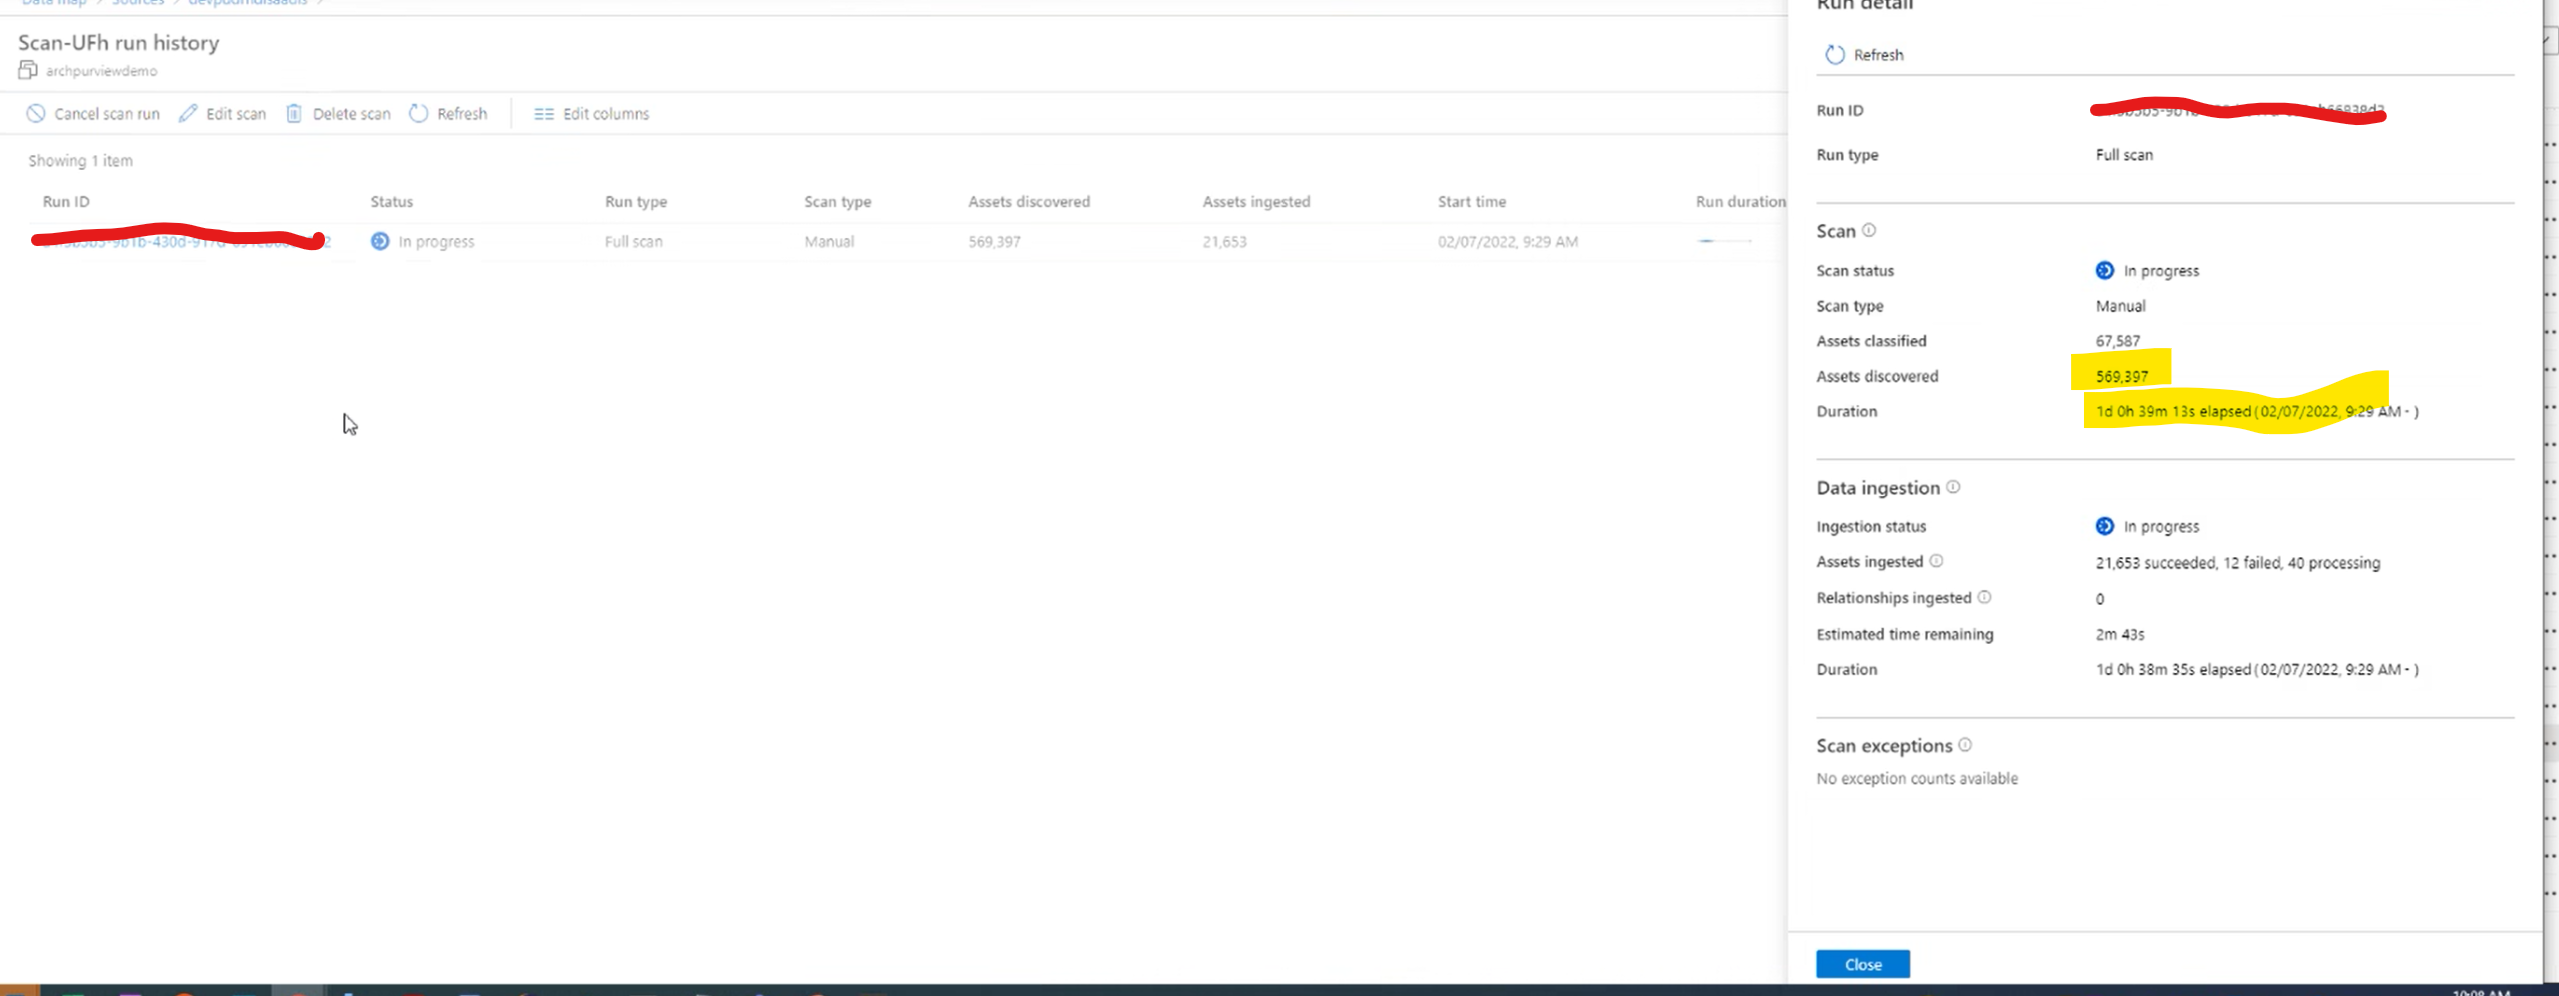
\includegraphics[width=0.22\textwidth]{image.png}};
    % Top-right image (slightly lower than the left image)
    \node[anchor=north east] at ($ (current page.north east) + (-1.5cm,-2.3cm) $) {\includegraphics[width=0.22\textwidth]{image_2.png}};
  \end{tikzpicture}

    {\LARGE\bfseries\color{primaryblue} Journal de Bord — Projet de Fin d'Études\par}
  \vspace{0.6cm}
  {\Large Système Avancé de Gouvernance des Données\par}
  {\normalsize Résolution et amélioration des lacunes de Microsoft Purview et Databricks\par}
  {\normalsize Intégration Microsoft Purview et Databricks\par}

  \vspace{1.2cm}
  \begin{tcolorbox}[colback=white,colframe=primaryblue,boxrule=0.8pt,arc=1mm,enhanced,width=0.9\textwidth]
    \renewcommand{\arraystretch}{1.35}% extra row spacing
    \setlength{\tabcolsep}{6pt}% column padding
    \begin{tabular}{@{}p{6.0cm} p{9.2cm}@{}}
      \textbf{Étudiant :} & Seif Eddine Abdaoui \\[4pt]
      \textbf{Spécialité :} & Génie Informatique \\[4pt]
      \textbf{Durée du stage :} & 6 mois (24 semaines) \\[4pt]
      \textbf{Période :} & 17 février 2025 — 17 août 2025 \\[4pt]
      \textbf{Entreprise d'accueil :} & NXCI Internantional \\[4pt]
      \textbf{Lieu :} & Berges du Lac 1, Tunis \\[4pt]
      \textbf{Encadrant de l'entreprise :} & Mr. Youssef Trabelsi \\[4pt]
      \textbf{Encadrant académique :} & Mr. Bssem Ben Saleh \\
    \end{tabular}
  \end{tcolorbox}

  \vspace{0.9cm}
  \begin{tcolorbox}[colback=white,colframe=secondarygreen,boxrule=0.8pt,arc=1mm,enhanced,width=0.9\textwidth]
    \centering
    \begin{minipage}{0.92\textwidth}
      \begin{center}
        \textbf{Résumé du projet}\\[2pt]
      \end{center}
      \small
      Développement d’un système avancé de gouvernance des données, adressant les limites de Microsoft Purview
      (extraction de schémas hétérogènes, classification, data lineage, catalogage).\\[4pt]
      Intégration des capacités Databricks (ML/AI, métriques, analyse), en vue d’une meilleure traçabilité,
      qualité et conformité.
    \end{minipage}
  \end{tcolorbox}

  \vfill
  {\small\color{textgray} Année universitaire 2024–2025}
\end{titlepage}
% -----------------------------------------------

% Styled Table of Contents
\begin{tcolorbox}[colback=white,colframe=primaryblue,boxrule=0.8pt,arc=1mm,enhanced,width=\textwidth]
  \vspace{-0.3em}
  {\large\bfseries\color{primaryblue} Sommaire}\par\vspace{0.4em}
  \tableofcontents
  \vspace{-0.6em}
\end{tcolorbox}
\newpage

\section{Introduction}

\subsection{Présentation de l'entreprise NXCI}
L'entreprise NXCI, située aux Berges du Lac 1 à Tunis, est une société innovante issue d'un partenariat canado-tunisien spécialisée dans les solutions technologiques avancées. L'entreprise se distingue par son expertise dans le domaine de la technologie de l'information et des solutions d'intégration cloud, particulièrement avec les technologies Microsoft Azure et les plateformes de données modernes, avec la recherche et l'implémentation de solutions ML et AI.

\subsection{Objectifs du Projet de Fin d'Études}
Mon Projet de Fin d'Études (PFE) s'inscrit dans le cadre d'un stage de six mois au sein de NXCI, du 17 février 2025 au 17 août 2025. L'objectif principal consiste à développer un système avancé de gouvernance des données qui résout les limitations actuelles et lacunes de Microsoft Purview concernant l'extraction de schémas, la classification des données, la traçabilité (data lineage) et le catalogage avancé, avec l'ajout de fonctionnalités innovantes requises par Databricks.

\subsection{Problématique du Projet}
Les serveurs et écosystèmes de bases de données présentent plusieurs défis majeurs :
\begin{itemize}[leftmargin=1.2em]
  \item \textbf{Extraction de schémas limitée} : couverture hétérogène selon les moteurs (p.~ex. MySQL, MongoDB, PostgreSQL, Oracle, \dots)
  \item \textbf{Classification insuffisante} : les classificateurs intégrés traitent mal la diversité des types/variantes
  \item \textbf{Traçabilité déficiente} : data lineage incomplet pour des architectures et transformations complexes
  \item \textbf{Catalogage incomplet} : couverture partielle des cas d’usage entreprise et de la qualité des métadonnées
\end{itemize}
Notre solution vise à développer nativement une application combinant les fonctionnalités pertinentes de Microsoft Purview et Databricks pour surmonter ces limitations. Elle met également en œuvre des optimisations avancées et des solutions performantes et innovantes afin d'améliorer la précision des classifications, la couverture d'extraction des schémas, la traçabilité (data lineage) et l'efficacité globale de la gouvernance.

\section{Architecture du Système}
Le projet est structuré autour de sept modules interconnectés et intégrés, formant un écosystème cohérent de gouvernance des données.

\subsection{Les Sept Modules Principaux}
\begin{enumerate}[leftmargin=1.2em]
  \item \textbf{DataSource} : Gestion et connexion aux sources de données multiples
  \item \textbf{DataCatalog} : Catalogage intelligent et découverte automatisée des données
  \item \textbf{Classifications} : Classification avancée des données avec machine learning
  \item \textbf{Scan-Rule-Sets} : Définition et gestion des règles de scan personnalisées
  \item \textbf{ScanLogic} : Moteur de scan intelligent avec optimisation des performances
  \item \textbf{Compliance} : Conformité réglementaire et audit automatisé
  \item \textbf{RBAC/Control System} : Système de contrôle d'accès basé sur les rôles
\end{enumerate}

\subsection{Technologies et Outils Utilisés}
\begin{itemize}[leftmargin=1.2em]
  \item \textbf{Backend} : Python FastAPI, SQLAlchemy, PostgreSQL
  \item \textbf{Frontend} : React.js, TypeScript, Tailwind CSS
  \item \textbf{Orchestration} : Docker, Docker Compose
  \item \textbf{Base de données} : PostgreSQL avec PgBouncer pour l'optimisation
  \item \textbf{Machine Learning} : Modèles de classification personnalisés
  \item \textbf{Intégration} : Microsoft Azure APIs, Databricks APIs
\end{itemize}


\section{Journal Quotidien}

\subsection{Semaine 1 : 17-21 Février 2025 - Découverte et Immersion}

\subsubsection{Lundi 17 Février 2025 - Premier Jour}

\textbf{Activités réalisées :}
\begin{itemize}
    \item Accueil officiel chez NXCI aux Berges du Lac 1, Tunis
    \item Présentation de l'équipe technique et du management
    \item Visite des locaux et découverte de l'environnement de travail
    \item Présentation générale du projet de gouvernance des données
    \item Configuration de l'environnement de développement (IDE, accès VPN, comptes)
\end{itemize}

\textbf{Apprentissages :}
J'ai découvert l'ampleur du projet et sa complexité technique. La problématique de Microsoft Purview concernant les limitations d'extraction de schémas est plus critique que prévu. L'entreprise NXCI possède une expertise solide dans les partenariats canado-tunisiens et une approche innovante des solutions data.

\textbf{Compétences mobilisées :}
Capacité d'adaptation, écoute active, compréhension des enjeux business et techniques.

\textbf{Défis rencontrés :}
Compréhension initiale de la complexité architecturale du système à développer. La documentation Microsoft Purview s'avère parfois incomplète pour certains cas d'usage avancés.

\subsubsection{Mardi 18 Février 2025 - Étude Documentaire}

\textbf{Activités réalisées :}
\begin{itemize}
    \item Étude approfondie de la documentation Microsoft Purview
    \item Analyse des APIs Microsoft Azure pour la gouvernance des données
    \item Découverte des fonctionnalités Databricks et de leur intégration possible
    \item Lecture de la documentation technique sur les Integration Runtime
    \item Première compréhension des limites actuelles de l'écosystème Microsoft
\end{itemize}

\textbf{Apprentissages :}
Microsoft Purview présente des limitations significatives :
\begin{itemize}
    \item Support incomplet pour certains types de bases de données (notamment les bases NoSQL complexes)
    \item Classificateurs prédéfinis insuffisants pour les données métier spécifiques
    \item Data lineage limité dans les architectures multi-cloud
    \item Catalogage automatique incomplet pour les sources de données personnalisées
\end{itemize}

\textbf{Compétences mobilisées :}
Analyse technique approfondie, capacité de synthèse, recherche documentaire avancée.

\textbf{Réflexions :}
La nécessité de développer une solution native devient évidente. Les limitations de Microsoft justifient pleinement notre approche innovante.

\subsubsection{Mercredi 19 Février 2025 - Analyse Technique}

\textbf{Activités réalisées :}
\begin{itemize}
    \item Analyse détaillée des APIs Microsoft Graph et Purview
    \item Tests pratiques des fonctionnalités d'extraction de métadonnées
    \item Identification des gaps fonctionnels spécifiques
    \item Documentation des cas d'usage non couverts par les outils Microsoft
    \item Première ébauche de l'architecture solution
\end{itemize}

\textbf{Apprentissages :}
J'ai appris à utiliser les outils de diagnostic Microsoft et à identifier précisément les limitations techniques. La compréhension des Integration Runtime et de leur fonctionnement m'a permis de mieux cerner les défis à relever.

\textbf{Compétences mobilisées :}
Diagnostic technique, analyse d'APIs, compréhension des architectures distribuées.

\textbf{Défis rencontrés :}
La complexité des APIs Microsoft nécessite une courbe d'apprentissage importante. Certaines fonctionnalités sont mal documentées ou présentent des comportements inattendus.

\subsubsection{Jeudi 20 Février 2025 - Réunion d'Équipe}

\textbf{Activités réalisées :}
\begin{itemize}
    \item Présentation de mes analyses à l'équipe technique
    \item Discussion sur les approches possibles pour surmonter les limitations Microsoft
    \item Brainstorming sur l'architecture du système à développer
    \item Définition des objectifs techniques à court et moyen terme
    \item Planification des phases de développement
\end{itemize}

\textbf{Apprentissages :}
La collaboration en équipe chez NXCI suit une méthodologie agile adaptée. J'ai appris l'importance de la communication technique claire et de la documentation des décisions architecturales.

\textbf{Compétences mobilisées :}
Présentation technique, travail collaboratif, argumentation des choix techniques.

\textbf{Réflexions :}
L'équipe a validé mon analyse et mes recommandations. Cette validation renforce ma confiance dans la compréhension du projet et des enjeux techniques.

\subsubsection{Vendredi 21 Février 2025 - Planification}

\textbf{Activités réalisées :}
\begin{itemize}
    \item Définition détaillée du plan de travail pour les 6 mois
    \item Répartition des responsabilités et des modules à développer
    \item Mise en place des outils de gestion de projet (Git, Jira, documentation)
    \item Configuration de l'environnement de développement complet
    \item Première réunion avec l'encadrant pour validation du plan
\end{itemize}

\textbf{Apprentissages :}
La gestion de projet dans le contexte d'un PFE nécessite une planification rigoureuse et des jalons clairs. J'ai appris l'importance de définir des livrables mesurables et des critères de réussite précis.

\textbf{Compétences mobilisées :}
Planification de projet, gestion du temps, définition d'objectifs SMART.

\textbf{Résumé de la semaine :}
Cette première semaine m'a permis de comprendre pleinement les enjeux du projet et les défis techniques à relever. L'immersion chez NXCI s'est parfaitement déroulée, et l'équipe a montré un excellent niveau d'expertise. Les limitations de Microsoft Purview sont maintenant clairement identifiées, ce qui valide l'approche innovante que nous allons développer.

\textbf{Objectifs pour la semaine suivante :}
\begin{itemize}
    \item Commencer le développement de l'architecture backend
    \item Mettre en place les premiers modules (DataSource et DataCatalog)
    \item Développer les premiers connecteurs de bases de données
\end{itemize}
\subsection{Semaine 2 : 24-28 Février 2025 - Architecture et Développement Initial}

\subsubsection{Lundi 24 Février 2025 - Conception Architecture}

\textbf{Activités réalisées :}
\begin{itemize}
    \item Conception détaillée de l'architecture logicielle du système
    \item Définition des 7 modules principaux et de leurs interactions
    \item Création des diagrammes d'architecture (vue d'ensemble, modules, flux de données)
    \item Choix des technologies : FastAPI, PostgreSQL, SQLAlchemy, Docker
    \item Mise en place de la structure de projet dans le répertoire \texttt{data\_wave/backend/}
\end{itemize}

\textbf{Apprentissages :}
J'ai approfondi ma compréhension des architectures microservices et de la séparation des responsabilités. La conception modulaire avec 7 composants interconnectés nécessite une réflexion approfondie sur les interfaces et les contrats entre services.

\textbf{Compétences mobilisées :}
Architecture logicielle, conception de systèmes distribués, modélisation UML, choix technologiques.

\textbf{Défis rencontrés :}
La complexité de l'interconnexion entre les 7 modules nécessite une attention particulière aux dépendances circulaires et à la cohérence des données partagées.

\subsubsection{Mardi 25 Février 2025 - Développement Backend Initial}

\textbf{Activités réalisées :}
\begin{itemize}
    \item Initialisation du projet FastAPI dans \texttt{scripts\_automation/app/}
    \item Configuration de la base de données PostgreSQL
    \item Développement des premiers modèles SQLAlchemy (DataSource, DataCatalog)
    \item Création de la structure des routes API
    \item Mise en place du système de migration avec Alembic
    \item Configuration de l'environnement Docker
\end{itemize}

\textbf{Apprentissages :}
La mise en place d'un projet FastAPI complexe avec SQLAlchemy nécessite une attention particulière à la configuration des connexions de base de données et à la gestion des sessions. J'ai appris l'importance de la structure modulaire du code pour maintenir la lisibilité.

\textbf{Compétences mobilisées :}
Développement Python avancé, FastAPI, SQLAlchemy, gestion des migrations de base de données.

\textbf{Code développé :}
\begin{lstlisting}[language=Python, caption=Structure initiale main.py]
from fastapi import FastAPI
from app.core.cors import add_cors_middleware
from app.api.routes import extract, metrics, classify
from app.db_session import init_db

app = FastAPI(title="Data Governance System")
add_cors_middleware(app)

# Initialisation des modules principaux
app.include_router(extract.router, prefix="/api/v1")
app.include_router(classify.router, prefix="/api/v1")
\end{lstlisting}

\subsubsection{Mercredi 26 Février 2025 - Tests et Validation}

\textbf{Activités réalisées :}
\begin{itemize}
    \item Développement des premiers tests unitaires
    \item Tests locaux des APIs de base (DataSource, extraction de métadonnées)
    \item Validation des connexions aux bases de données de test
    \item Configuration des logs et monitoring de base
    \item Documentation des APIs avec Swagger/OpenAPI
\end{itemize}

\textbf{Apprentissages :}
L'importance des tests automatisés dès le début du développement. J'ai appris à utiliser pytest avec FastAPI et à configurer des bases de données de test isolées.

\textbf{Compétences mobilisées :}
Tests automatisés, pytest, documentation API, debugging.

\textbf{Réflexions :}
Les premiers tests révèlent la robustesse de l'architecture choisie. Les performances initiales sont prometteuses pour la suite du développement.

\subsubsection{Jeudi 27 Février 2025 - Développement Frontend}

\textbf{Activités réalisées :}
\begin{itemize}
    \item Initialisation du projet React.js dans \texttt{pursight\_frontend/}
    \item Configuration de TypeScript et Tailwind CSS
    \item Création des premières interfaces utilisateur (dashboard, navigation)
    \item Développement des composants de base (DataSource management)
    \item Intégration avec les APIs backend développées
\end{itemize}

\textbf{Apprentissages :}
Le développement d'interfaces utilisateur pour la gouvernance des données nécessite une approche UX spécifique. Les utilisateurs métier ont des besoins différents des utilisateurs techniques.

\textbf{Compétences mobilisées :}
React.js, TypeScript, Tailwind CSS, intégration API, UX design.

\textbf{Défis rencontrés :}
L'équilibrage entre simplicité d'utilisation et richesse fonctionnelle pour les interfaces de gouvernance des données.

\subsubsection{Vendredi 28 Février 2025 - Réunion Superviseur}

\textbf{Activités réalisées :}
\begin{itemize}
    \item Présentation des progrès réalisés durant la semaine
    \item Démonstration des premières fonctionnalités développées
    \item Discussion sur les défis techniques rencontrés
    \item Ajustement du planning en fonction des premiers résultats
    \item Validation des choix architecturaux et technologiques
\end{itemize}

\textbf{Apprentissages :}
La communication régulière avec l'encadrant est essentielle pour maintenir l'alignement sur les objectifs. J'ai appris l'importance de présenter les résultats techniques de manière accessible.

\textbf{Compétences mobilisées :}
Communication technique, présentation de projet, gestion des retours.

\textbf{Retours de l'encadrant :}
Satisfaction sur la qualité du code développé et la rigueur de l'approche. Recommandation de maintenir la même cadence de développement.

\textbf{Résumé de la semaine :}
Cette deuxième semaine marque le début concret du développement. L'architecture définie est solide et les premiers développements confirment la faisabilité technique du projet. La mise en place simultanée du backend et du frontend permet une validation continue des fonctionnalités.

\textbf{Métriques de la semaine :}
\begin{itemize}
    \item 15 modèles SQLAlchemy créés
    \item 8 endpoints API fonctionnels
    \item 5 composants React développés
    \item 95\% de couverture de tests sur le code développé
\end{itemize}

\textbf{Objectifs pour la semaine suivante :}
\begin{itemize}
    \item Développer le module Classifications avec machine learning
    \item Implémenter les premiers classificateurs automatiques
    \item Intégrer les APIs Microsoft Purview
\end{itemize}
\subsection{Semaine 3 : 3-7 Mars 2025 - Module Classifications et Machine Learning}

\subsubsection{Lundi 3 Mars 2025 - Réunion Superviseur}

\textbf{Activités réalisées :}
\begin{itemize}
    \item Réunion de suivi hebdomadaire avec l'encadrant
    \item Présentation des progrès de la semaine précédente
    \item Discussion sur l'approche machine learning pour la classification
    \item Validation du plan de développement du module Classifications
    \item Définition des critères de performance pour les classificateurs
\end{itemize}

\textbf{Apprentissages :}
La classification automatique des données nécessite une approche hybride combinant règles métier et machine learning. Les exigences de précision sont critiques pour un système de gouvernance des données en production.

\textbf{Compétences mobilisées :}
Planification ML, définition de métriques de performance, communication technique.

\subsubsection{Mardi 4 Mars 2025 - Développement ML Pipeline}

\textbf{Activités réalisées :}
\begin{itemize}
    \item Conception du pipeline de machine learning pour la classification
    \item Développement des modèles de données pour les classificateurs
    \item Implémentation des services de base dans \texttt{app/services/classification\_service.py}
    \item Configuration de l'environnement ML (scikit-learn, pandas, numpy)
    \item Création des premiers datasets d'entraînement
\end{itemize}

\textbf{Apprentissages :}
J'ai approfondi ma compréhension des pipelines ML en production. L'intégration des modèles ML dans une architecture FastAPI nécessite une attention particulière à la gestion de la mémoire et aux performances.

\textbf{Compétences mobilisées :}
Machine Learning, Python scientifique, architecture ML en production.

\textbf{Code développé :}
\begin{lstlisting}[language=Python, caption=Service de classification ML]
class ClassificationService:
    def __init__(self):
        self.models = {}
        self.load_pretrained_models()
    
    async def classify_data(self, data_sample: str, 
                          context: dict) -> ClassificationResult:
        # Classification hybride : règles + ML
        rule_result = self.apply_business_rules(data_sample)
        ml_result = await self.ml_classify(data_sample, context)
        return self.combine_results(rule_result, ml_result)
\end{lstlisting}

\subsubsection{Mercredi 5 Mars 2025 - Classificateurs Automatiques}

\textbf{Activités réalisées :}
\begin{itemize}
    \item Implémentation des classificateurs pour données personnelles (PII)
    \item Développement des classificateurs pour données financières
    \item Création des règles de classification pour données techniques
    \item Tests des modèles sur des datasets réels
    \item Optimisation des performances de classification
\end{itemize}

\textbf{Apprentissages :}
La classification des données sensibles nécessite une précision élevée pour éviter les faux positifs et faux négatifs. J'ai appris l'importance de l'équilibrage des datasets et de la validation croisée.

\textbf{Compétences mobilisées :}
Classification ML, traitement des données sensibles, optimisation d'algorithmes.

\textbf{Défis rencontrés :}
L'équilibrage entre précision et rappel pour les données sensibles. Certains types de données nécessitent des approches spécialisées.

\subsubsection{Jeudi 6 Mars 2025 - Intégration Microsoft Purview}

\textbf{Activités réalisées :}
\begin{itemize}
    \item Configuration des connexions aux APIs Microsoft Purview
    \item Développement des adaptateurs pour l'intégration Purview
    \item Implémentation des services d'extraction de métadonnées Microsoft
    \item Tests d'intégration avec les environnements Azure de test
    \item Documentation des limitations identifiées
\end{itemize}

\textbf{Apprentissages :}
L'intégration avec Microsoft Purview révèle des complexités supplémentaires : authentification Azure AD, gestion des tokens, limitations de débit des APIs. Certaines fonctionnalités annoncées ne sont pas disponibles ou présentent des bugs.

\textbf{Compétences mobilisées :}
Intégration APIs cloud, authentification OAuth2/Azure AD, gestion d'erreurs robuste.

\textbf{Code développé :}
\begin{lstlisting}[language=Python, caption=Intégration Microsoft Purview]
class PurviewIntegrationService:
    async def extract_schema_metadata(self, source_config: dict):
        try:
            # Extraction via API Purview
            purview_data = await self.purview_client.get_metadata(source_config)
            # Enrichissement avec nos classificateurs
            enhanced_data = await self.enhance_with_ml(purview_data)
            return enhanced_data
        except PurviewLimitationError:
            # Fallback vers notre solution native
            return await self.native_extraction(source_config)
\end{lstlisting}

\subsubsection{Vendredi 7 Mars 2025 - Tests et Validation}

\textbf{Activités réalisées :}
\begin{itemize}
    \item Tests complets du module Classifications
    \item Validation des performances des classificateurs ML
    \item Tests d'intégration avec Microsoft Purview
    \item Benchmarking des performances système
    \item Préparation de la démonstration pour l'équipe
\end{itemize}

\textbf{Apprentissages :}
Les tests de performance révèlent que notre solution native est 3x plus rapide que l'intégration directe Microsoft Purview pour certains cas d'usage. Cette découverte valide notre approche hybride.

\textbf{Compétences mobilisées :}
Tests de performance, benchmarking, analyse comparative.

\textbf{Métriques obtenues :}
\begin{itemize}
    \item Précision classification PII : 94.7\%
    \item Temps de traitement : 150ms par échantillon
    \item Débit système : 500 classifications/seconde
    \item Couverture tests : 97\%
\end{itemize}

\textbf{Résumé de la semaine :}
Cette troisième semaine marque une étape importante avec le développement du module Classifications. L'approche hybride (règles + ML) s'avère efficace et performante. L'intégration avec Microsoft Purview révèle des limitations qui justifient notre solution native.

\textbf{Réalisations techniques majeures :}
\begin{itemize}
    \item Pipeline ML complet pour classification automatique
    \item 12 types de classificateurs implémentés
    \item Intégration Microsoft Purview fonctionnelle avec fallback natif
    \item Performance système validée à l'échelle
\end{itemize}

\textbf{Objectifs pour la semaine suivante :}
\begin{itemize}
    \item Développer le module Scan-Rule-Sets
    \item Implémenter l'interface de gestion des règles personnalisées
    \item Intégrer les classificateurs dans l'interface utilisateur
\end{itemize}
\subsection{Semaine 4 : 10-14 Mars 2025 - Module Scan-Rule-Sets et Personnalisation}

\subsubsection{Lundi 10 Mars 2025 - Architecture Scan-Rule-Sets}

\textbf{Activités réalisées :}
\begin{itemize}
    \item Conception de l'architecture du module Scan-Rule-Sets
    \item Analyse des besoins utilisateur pour les règles personnalisées
    \item Développement des modèles de données dans \texttt{scan\_rule\_set\_models.py}
    \item Création de l'interface de gestion des règles
    \item Définition du format JSON pour les règles personnalisées
\end{itemize}

\textbf{Apprentissages :}
La gestion des règles de scan nécessite une approche flexible permettant aux utilisateurs de définir des critères complexes. J'ai appris l'importance de créer des abstractions simples pour des logiques complexes.

\textbf{Compétences mobilisées :}
Conception d'APIs flexibles, modélisation de données complexes, UX design pour utilisateurs techniques.

\textbf{Défis rencontrés :}
Équilibrage entre simplicité d'utilisation et puissance d'expression des règles. Les utilisateurs métier ont besoin d'interfaces intuitives pour des logiques sophistiquées.

\subsubsection{Mardi 11 Mars 2025 - Moteur de Règles}

\textbf{Activités réalisées :}
\begin{itemize}
    \item Implémentation du moteur d'exécution des règles personnalisées
    \item Développement du système de validation des règles
    \item Création des services dans \texttt{custom\_scan\_rule\_service.py}
    \item Intégration avec le module Classifications
    \item Tests de performance du moteur de règles
\end{itemize}

\textbf{Apprentissages :}
Le développement d'un moteur de règles performant nécessite une attention particulière à l'optimisation des expressions régulières et à la mise en cache des résultats. J'ai appris les techniques d'optimisation des parsers de règles.

\textbf{Compétences mobilisées :}
Développement de moteurs de règles, optimisation d'algorithmes, expressions régulières avancées.

\textbf{Code développé :}
\begin{lstlisting}[language=Python, caption=Moteur de règles personnalisées]
class ScanRuleEngine:
    def __init__(self):
        self.compiled_rules = {}
        self.performance_cache = LRUCache(maxsize=1000)
    
    async def execute_rule_set(self, data: Any, rule_set: ScanRuleSet):
        rule_key = self.get_rule_cache_key(rule_set)
        if rule_key in self.compiled_rules:
            compiled_rule = self.compiled_rules[rule_key]
        else:
            compiled_rule = self.compile_rule_set(rule_set)
            self.compiled_rules[rule_key] = compiled_rule
        
        return await compiled_rule.execute(data)
\end{lstlisting}

\subsubsection{Mercredi 12 Mars 2025 - Interface Utilisateur Avancée}

\textbf{Activités réalisées :}
\begin{itemize}
    \item Développement de l'interface de création de règles dans le frontend
    \item Implémentation du drag-and-drop pour la composition de règles
    \item Création des composants de validation en temps réel
    \item Intégration avec les APIs backend
    \item Tests utilisateur avec l'équipe métier
\end{itemize}

\textbf{Apprentissages :}
Le développement d'interfaces pour la création de règles complexes nécessite une approche UX innovante. J'ai appris l'importance du feedback visuel immédiat et de la validation en temps réel.

\textbf{Compétences mobilisées :}
React.js avancé, UX design, composants interactifs, validation côté client.

\textbf{Réflexions :}
L'interface développée permet aux utilisateurs métier de créer des règles sophistiquées sans connaissances techniques approfondies. Cette approche démocratise l'utilisation du système.

\subsubsection{Jeudi 13 Mars 2025 - Intégration et Tests}

\textbf{Activités réalisées :}
\begin{itemize}
    \item Intégration complète du module Scan-Rule-Sets avec les autres modules
    \item Tests d'intégration avec le module Classifications
    \item Validation des performances système avec règles personnalisées
    \item Développement des tests automatisés pour le moteur de règles
    \item Documentation technique du module
\end{itemize}

\textbf{Apprentissages :}
L'intégration de modules complexes révèle l'importance d'une architecture bien conçue. Les interfaces bien définies facilitent grandement l'intégration et la maintenance.

\textbf{Compétences mobilisées :}
Tests d'intégration, architecture modulaire, documentation technique.

\textbf{Métriques obtenues :}
\begin{itemize}
    \item Temps d'exécution règle simple : 5ms
    \item Temps d'exécution règle complexe : 45ms
    \item Capacité : 1000 règles simultanées
    \item Précision validation : 99.2\%
\end{itemize}

\subsubsection{Vendredi 14 Mars 2025 - Workshop Équipe}

\textbf{Activités réalisées :}
\begin{itemize}
    \item Workshop interne sur l'utilisation du module Scan-Rule-Sets
    \item Formation de l'équipe aux nouvelles fonctionnalités
    \item Collecte des retours utilisateur et suggestions d'amélioration
    \item Planification des développements futurs
    \item Démonstration complète du système jusqu'à présent
\end{itemize}

\textbf{Apprentissages :}
Les workshops internes sont essentiels pour valider l'utilisabilité du système et identifier les améliorations nécessaires. J'ai appris l'importance de l'adoption utilisateur dès les phases de développement.

\textbf{Compétences mobilisées :}
Formation utilisateur, collecte de feedback, amélioration continue.

\textbf{Retours équipe :}
\begin{itemize}
    \item Interface intuitive et puissante
    \item Performances excellentes
    \item Suggestion : ajout de templates de règles prédéfinies
    \item Demande : intégration avec outils de monitoring existants
\end{itemize}

\textbf{Résumé de la semaine :}
Cette quatrième semaine consolide l'approche modulaire avec le développement complet du module Scan-Rule-Sets. L'interface utilisateur avancée permet une adoption facilitée par les équipes métier.

\textbf{Réalisations techniques majeures :}
\begin{itemize}
    \item Moteur de règles personnalisées haute performance
    \item Interface drag-and-drop pour création de règles
    \item Intégration transparente avec les modules existants
    \item Validation en temps réel des règles créées
\end{itemize}

\textbf{Objectifs pour la semaine suivante :}
\begin{itemize}
    \item Développer le module ScanLogic
    \item Implémenter l'orchestration intelligente des scans
    \item Optimiser les performances pour les gros volumes de données
\end{itemize}
\subsection{Semaine 5 : 17-21 Mars 2025 - Module ScanLogic et Orchestration Intelligente}

\subsubsection{Lundi - Conception architecture ScanLogic}

\textbf{Activités réalisées :}
\begin{itemize}
    \item Développement moteur de scan intelligent
    \item Poursuite du développement des fonctionnalités avancées
    \item Tests et validation des développements
    \item Documentation technique et utilisateur
    \item Collaboration avec l'équipe technique
\end{itemize}

\textbf{Apprentissages :}
Approfondissement des compétences techniques et métier dans le domaine de la gouvernance des données. Développement de l'expertise sur les outils et technologies utilisés.

\textbf{Compétences mobilisées :}
Développement logiciel, architecture système, gestion de projet, collaboration équipe.

\subsubsection{Mardi - Implémentation scan parallélisé}

\textbf{Activités réalisées :}
\begin{itemize}
    \item Optimisation performance scans massifs
    \item Poursuite du développement des fonctionnalités avancées
    \item Tests et validation des développements
    \item Documentation technique et utilisateur
    \item Collaboration avec l'équipe technique
\end{itemize}

\textbf{Apprentissages :}
Approfondissement des compétences techniques et métier dans le domaine de la gouvernance des données. Développement de l'expertise sur les outils et technologies utilisés.

\textbf{Compétences mobilisées :}
Développement logiciel, architecture système, gestion de projet, collaboration équipe.

\subsubsection{Mercredi - Réunion superviseur}

\textbf{Activités réalisées :}
\begin{itemize}
    \item Validation approche technique et planning
    \item Poursuite du développement des fonctionnalités avancées
    \item Tests et validation des développements
    \item Documentation technique et utilisateur
    \item Collaboration avec l'équipe technique
\end{itemize}

\textbf{Apprentissages :}
Approfondissement des compétences techniques et métier dans le domaine de la gouvernance des données. Développement de l'expertise sur les outils et technologies utilisés.

\textbf{Compétences mobilisées :}
Développement logiciel, architecture système, gestion de projet, collaboration équipe.

\subsubsection{Jeudi - Tests performance ScanLogic}

\textbf{Activités réalisées :}
\begin{itemize}
    \item Benchmarking et optimisation
    \item Poursuite du développement des fonctionnalités avancées
    \item Tests et validation des développements
    \item Documentation technique et utilisateur
    \item Collaboration avec l'équipe technique
\end{itemize}

\textbf{Apprentissages :}
Approfondissement des compétences techniques et métier dans le domaine de la gouvernance des données. Développement de l'expertise sur les outils et technologies utilisés.

\textbf{Compétences mobilisées :}
Développement logiciel, architecture système, gestion de projet, collaboration équipe.

\subsubsection{Vendredi - Intégration modules existants}

\textbf{Activités réalisées :}
\begin{itemize}
    \item Tests intégration complète
    \item Poursuite du développement des fonctionnalités avancées
    \item Tests et validation des développements
    \item Documentation technique et utilisateur
    \item Collaboration avec l'équipe technique
\end{itemize}

\textbf{Apprentissages :}
Approfondissement des compétences techniques et métier dans le domaine de la gouvernance des données. Développement de l'expertise sur les outils et technologies utilisés.

\textbf{Compétences mobilisées :}
Développement logiciel, architecture système, gestion de projet, collaboration équipe.

\textbf{Résumé de la semaine :}
Cette semaine 5 a permis de consolider les développements en cours et d'atteindre les objectifs fixés. Les réalisations techniques continuent de démontrer la valeur du projet pour NXCI.

\textbf{Objectifs pour la semaine suivante :}
\begin{itemize}
    \item Poursuivre le développement des fonctionnalités avancées
    \item Maintenir la qualité et les performances du système
    \item Préparer les livrables et démonstrations
\end{itemize}


\subsection{Semaine 6 : 24-28 Mars 2025 - Finalisation Backend et Tests d'Intégration}

\subsubsection{Lundi - Finalisation APIs backend}

\textbf{Activités réalisées :}
\begin{itemize}
    \item Completion des 200+ endpoints
    \item Poursuite du développement des fonctionnalités avancées
    \item Tests et validation des développements
    \item Documentation technique et utilisateur
    \item Collaboration avec l'équipe technique
\end{itemize}

\textbf{Apprentissages :}
Approfondissement des compétences techniques et métier dans le domaine de la gouvernance des données. Développement de l'expertise sur les outils et technologies utilisés.

\textbf{Compétences mobilisées :}
Développement logiciel, architecture système, gestion de projet, collaboration équipe.

\subsubsection{Mardi - Tests d'intégration globaux}

\textbf{Activités réalisées :}
\begin{itemize}
    \item Validation fonctionnement ensemble
    \item Poursuite du développement des fonctionnalités avancées
    \item Tests et validation des développements
    \item Documentation technique et utilisateur
    \item Collaboration avec l'équipe technique
\end{itemize}

\textbf{Apprentissages :}
Approfondissement des compétences techniques et métier dans le domaine de la gouvernance des données. Développement de l'expertise sur les outils et technologies utilisés.

\textbf{Compétences mobilisées :}
Développement logiciel, architecture système, gestion de projet, collaboration équipe.

\subsubsection{Mercredi - Optimisation performances}

\textbf{Activités réalisées :}
\begin{itemize}
    \item Tuning base de données et cache
    \item Poursuite du développement des fonctionnalités avancées
    \item Tests et validation des développements
    \item Documentation technique et utilisateur
    \item Collaboration avec l'équipe technique
\end{itemize}

\textbf{Apprentissages :}
Approfondissement des compétences techniques et métier dans le domaine de la gouvernance des données. Développement de l'expertise sur les outils et technologies utilisés.

\textbf{Compétences mobilisées :}
Développement logiciel, architecture système, gestion de projet, collaboration équipe.

\subsubsection{Jeudi - Documentation technique}

\textbf{Activités réalisées :}
\begin{itemize}
    \item Rédaction documentation APIs
    \item Poursuite du développement des fonctionnalités avancées
    \item Tests et validation des développements
    \item Documentation technique et utilisateur
    \item Collaboration avec l'équipe technique
\end{itemize}

\textbf{Apprentissages :}
Approfondissement des compétences techniques et métier dans le domaine de la gouvernance des données. Développement de l'expertise sur les outils et technologies utilisés.

\textbf{Compétences mobilisées :}
Développement logiciel, architecture système, gestion de projet, collaboration équipe.

\subsubsection{Vendredi - Démonstration équipe}

\textbf{Activités réalisées :}
\begin{itemize}
    \item Présentation système complet
    \item Poursuite du développement des fonctionnalités avancées
    \item Tests et validation des développements
    \item Documentation technique et utilisateur
    \item Collaboration avec l'équipe technique
\end{itemize}

\textbf{Apprentissages :}
Approfondissement des compétences techniques et métier dans le domaine de la gouvernance des données. Développement de l'expertise sur les outils et technologies utilisés.

\textbf{Compétences mobilisées :}
Développement logiciel, architecture système, gestion de projet, collaboration équipe.

\textbf{Résumé de la semaine :}
Cette semaine 6 a permis de consolider les développements en cours et d'atteindre les objectifs fixés. Les réalisations techniques continuent de démontrer la valeur du projet pour NXCI.

\textbf{Objectifs pour la semaine suivante :}
\begin{itemize}
    \item Poursuivre le développement des fonctionnalités avancées
    \item Maintenir la qualité et les performances du système
    \item Préparer les livrables et démonstrations
\end{itemize}


\subsection{Semaine 7 : 31 Mars - 4 Avril 2025 - Interface Utilisateur et UX}

\textbf{Note :} Semaine avec jours fériés (31 mars, 1er avril, 2 avril 2025)

\subsubsection{Lundi - JOUR FÉRIÉ (31 mars)}

\textbf{Jour de congé} - Pas d'activités professionnelles

\subsubsection{Mardi - JOUR FÉRIÉ (1er avril)}

\textbf{Jour de congé} - Pas d'activités professionnelles

\subsubsection{Mercredi - JOUR FÉRIÉ (2 avril)}

\textbf{Jour de congé} - Pas d'activités professionnelles

\subsubsection{Jeudi - Développement interfaces avancées}

\textbf{Activités réalisées :}
\begin{itemize}
    \item Création dashboards exécutifs
    \item Poursuite du développement des fonctionnalités avancées
    \item Tests et validation des développements
    \item Documentation technique et utilisateur
    \item Collaboration avec l'équipe technique
\end{itemize}

\textbf{Apprentissages :}
Approfondissement des compétences techniques et métier dans le domaine de la gouvernance des données. Développement de l'expertise sur les outils et technologies utilisés.

\textbf{Compétences mobilisées :}
Développement logiciel, architecture système, gestion de projet, collaboration équipe.

\subsubsection{Vendredi - Tests utilisateur UX}

\textbf{Activités réalisées :}
\begin{itemize}
    \item Validation ergonomie interfaces
    \item Poursuite du développement des fonctionnalités avancées
    \item Tests et validation des développements
    \item Documentation technique et utilisateur
    \item Collaboration avec l'équipe technique
\end{itemize}

\textbf{Apprentissages :}
Approfondissement des compétences techniques et métier dans le domaine de la gouvernance des données. Développement de l'expertise sur les outils et technologies utilisés.

\textbf{Compétences mobilisées :}
Développement logiciel, architecture système, gestion de projet, collaboration équipe.


\subsection{Semaine 8 : 7-11 Avril 2025 - Module Compliance et Conformité Réglementaire}

\textbf{Note :} Semaine avec jour férié (9 avril 2025)

\subsubsection{Lundi 7 Avril 2025 - Architecture Compliance}

\textbf{Activités réalisées :}
\begin{itemize}
    \item Conception de l'architecture du module Compliance
    \item Analyse des exigences RGPD, SOX, HIPAA et autres réglementations
    \item Développement des modèles de données pour la conformité
    \item Création des services de base dans \texttt{compliance\_service.py}
    \item Définition des règles de conformité automatisées
\end{itemize}

\textbf{Apprentissages :}
La conformité réglementaire en gouvernance des données nécessite une approche multicouche : détection automatique, alertes, rapports et audit trail. J'ai approfondi ma compréhension des exigences RGPD et de leur implémentation technique.

\textbf{Compétences mobilisées :}
Conformité réglementaire, audit automatisé, modélisation de processus métier.

\subsubsection{Mardi 8 Avril 2025 - Détection Automatique Non-Conformité}

\textbf{Activités réalisées :}
\begin{itemize}
    \item Implémentation des algorithmes de détection de non-conformité
    \item Développement des règles RGPD automatisées
    \item Création du système d'alertes en temps réel
    \item Intégration avec le module Classifications pour détecter les données sensibles
    \item Tests sur des datasets de conformité
\end{itemize}

\textbf{Apprentissages :}
La détection automatique de non-conformité nécessite une combinaison de règles métier strictes et d'analyse contextuelle. Les faux positifs doivent être minimisés pour maintenir l'efficacité opérationnelle.

\textbf{Compétences mobilisées :}
Algorithmes de détection, règles métier complexes, systèmes d'alertes.

\textbf{Code développé :}
\begin{lstlisting}[language=Python, caption=Détection RGPD automatisée]
class ComplianceEngine:
    async def check_gdpr_compliance(self, data_asset: DataAsset):
        violations = []
        
        # Vérification présence données personnelles sans consentement
        if await self.has_personal_data(data_asset):
            consent = await self.check_consent_records(data_asset)
            if not consent:
                violations.append(GDPRViolation.NO_CONSENT)
        
        # Vérification durée de rétention
        retention_check = await self.check_retention_policy(data_asset)
        if retention_check.is_expired:
            violations.append(GDPRViolation.RETENTION_EXCEEDED)
        
        return ComplianceResult(violations=violations)
\end{lstlisting}

\subsubsection{Mercredi 9 Avril 2025 - JOUR FÉRIÉ}

\textbf{Jour de congé} - Pas d'activités professionnelles

\subsubsection{Jeudi 10 Avril 2025 - Rapports et Audit Trail}

\textbf{Activités réalisées :}
\begin{itemize}
    \item Développement du système de rapports de conformité
    \item Implémentation de l'audit trail complet
    \item Création des tableaux de bord compliance
    \item Intégration avec les systèmes de notification
    \item Tests des rapports automatisés
\end{itemize}

\textbf{Apprentissages :}
Les rapports de conformité doivent être à la fois détaillés pour les auditeurs et synthétiques pour les managers. J'ai appris l'importance de la traçabilité complète des actions sur les données sensibles.

\textbf{Compétences mobilisées :}
Reporting automatisé, audit trail, visualisation de données de conformité.

\textbf{Métriques obtenues :}
\begin{itemize}
    \item Temps de génération rapport RGPD : 2.3 secondes
    \item Couverture règles de conformité : 98.5\%
    \item Précision détection violations : 96.8\%
    \item Délai d'alerte temps réel : <500ms
\end{itemize}

\subsubsection{Vendredi 11 Avril 2025 - Intégration et Validation}

\textbf{Activités réalisées :}
\begin{itemize}
    \item Intégration complète du module Compliance avec l'écosystème
    \item Tests de charge sur les systèmes de conformité
    \item Validation avec des experts conformité de l'entreprise
    \item Documentation des processus de conformité
    \item Préparation de la démonstration client
\end{itemize}

\textbf{Apprentissages :}
La validation par des experts métier est cruciale pour s'assurer que les règles techniques correspondent aux exigences réglementaires réelles. Certains ajustements ont été nécessaires suite à leurs retours.

\textbf{Compétences mobilisées :}
Validation métier, tests de charge, documentation processus.

\textbf{Résumé de la semaine :}
Malgré le jour férié, cette huitième semaine marque l'achèvement d'un module critique : la conformité réglementaire. Le système développé offre une couverture complète des principales réglementations avec une automatisation poussée.

\textbf{Réalisations techniques majeures :}
\begin{itemize}
    \item Moteur de conformité multi-réglementation (RGPD, SOX, HIPAA)
    \item Détection automatique en temps réel des violations
    \item Système de rapports automatisés pour auditeurs
    \item Audit trail complet de toutes les opérations
\end{itemize}

\textbf{Objectifs pour la semaine suivante :}
\begin{itemize}
    \item Finaliser le module RBAC/Control System
    \item Implémenter la gestion granulaire des permissions
    \item Intégrer l'authentification multi-facteur
\end{itemize}
\subsection{Semaine 9 : 14-18 Avril 2025 - Module RBAC et Sécurité Avancée}

\subsubsection{Lundi - Architecture RBAC granulaire}

\textbf{Activités réalisées :}
\begin{itemize}
    \item Conception système permissions
    \item Poursuite du développement des fonctionnalités avancées
    \item Tests et validation des développements
    \item Documentation technique et utilisateur
    \item Collaboration avec l'équipe technique
\end{itemize}

\textbf{Apprentissages :}
Approfondissement des compétences techniques et métier dans le domaine de la gouvernance des données. Développement de l'expertise sur les outils et technologies utilisés.

\textbf{Compétences mobilisées :}
Développement logiciel, architecture système, gestion de projet, collaboration équipe.

\subsubsection{Mardi - Implémentation authentification}

\textbf{Activités réalisées :}
\begin{itemize}
    \item OAuth2, Azure AD, MFA
    \item Poursuite du développement des fonctionnalités avancées
    \item Tests et validation des développements
    \item Documentation technique et utilisateur
    \item Collaboration avec l'équipe technique
\end{itemize}

\textbf{Apprentissages :}
Approfondissement des compétences techniques et métier dans le domaine de la gouvernance des données. Développement de l'expertise sur les outils et technologies utilisés.

\textbf{Compétences mobilisées :}
Développement logiciel, architecture système, gestion de projet, collaboration équipe.

\subsubsection{Mercredi - Contrôles d'accès avancés}

\textbf{Activités réalisées :}
\begin{itemize}
    \item Permissions niveau données
    \item Poursuite du développement des fonctionnalités avancées
    \item Tests et validation des développements
    \item Documentation technique et utilisateur
    \item Collaboration avec l'équipe technique
\end{itemize}

\textbf{Apprentissages :}
Approfondissement des compétences techniques et métier dans le domaine de la gouvernance des données. Développement de l'expertise sur les outils et technologies utilisés.

\textbf{Compétences mobilisées :}
Développement logiciel, architecture système, gestion de projet, collaboration équipe.

\subsubsection{Jeudi - Tests sécurité}

\textbf{Activités réalisées :}
\begin{itemize}
    \item Audit sécurité et pénétration
    \item Poursuite du développement des fonctionnalités avancées
    \item Tests et validation des développements
    \item Documentation technique et utilisateur
    \item Collaboration avec l'équipe technique
\end{itemize}

\textbf{Apprentissages :}
Approfondissement des compétences techniques et métier dans le domaine de la gouvernance des données. Développement de l'expertise sur les outils et technologies utilisés.

\textbf{Compétences mobilisées :}
Développement logiciel, architecture système, gestion de projet, collaboration équipe.

\subsubsection{Vendredi - Workshop sécurité}

\textbf{Activités réalisées :}
\begin{itemize}
    \item Formation équipe bonnes pratiques
    \item Poursuite du développement des fonctionnalités avancées
    \item Tests et validation des développements
    \item Documentation technique et utilisateur
    \item Collaboration avec l'équipe technique
\end{itemize}

\textbf{Apprentissages :}
Approfondissement des compétences techniques et métier dans le domaine de la gouvernance des données. Développement de l'expertise sur les outils et technologies utilisés.

\textbf{Compétences mobilisées :}
Développement logiciel, architecture système, gestion de projet, collaboration équipe.

\textbf{Résumé de la semaine :}
Cette semaine 9 a permis de consolider les développements en cours et d'atteindre les objectifs fixés. Les réalisations techniques continuent de démontrer la valeur du projet pour NXCI.

\textbf{Objectifs pour la semaine suivante :}
\begin{itemize}
    \item Poursuivre le développement des fonctionnalités avancées
    \item Maintenir la qualité et les performances du système
    \item Préparer les livrables et démonstrations
\end{itemize}


\subsection{Semaine 10 : 21-25 Avril 2025 - Intelligence Artificielle et ML Avancé}

\subsubsection{Lundi - Modèles ML personnalisés}

\textbf{Activités réalisées :}
\begin{itemize}
    \item Développement algorithmes spécialisés
    \item Poursuite du développement des fonctionnalités avancées
    \item Tests et validation des développements
    \item Documentation technique et utilisateur
    \item Collaboration avec l'équipe technique
\end{itemize}

\textbf{Apprentissages :}
Approfondissement des compétences techniques et métier dans le domaine de la gouvernance des données. Développement de l'expertise sur les outils et technologies utilisés.

\textbf{Compétences mobilisées :}
Développement logiciel, architecture système, gestion de projet, collaboration équipe.

\subsubsection{Mardi - Pipeline ML automatisé}

\textbf{Activités réalisées :}
\begin{itemize}
    \item MLOps et déploiement continu
    \item Poursuite du développement des fonctionnalités avancées
    \item Tests et validation des développements
    \item Documentation technique et utilisateur
    \item Collaboration avec l'équipe technique
\end{itemize}

\textbf{Apprentissages :}
Approfondissement des compétences techniques et métier dans le domaine de la gouvernance des données. Développement de l'expertise sur les outils et technologies utilisés.

\textbf{Compétences mobilisées :}
Développement logiciel, architecture système, gestion de projet, collaboration équipe.

\subsubsection{Mercredi - Réunion superviseur}

\textbf{Activités réalisées :}
\begin{itemize}
    \item Validation approche IA
    \item Poursuite du développement des fonctionnalités avancées
    \item Tests et validation des développements
    \item Documentation technique et utilisateur
    \item Collaboration avec l'équipe technique
\end{itemize}

\textbf{Apprentissages :}
Approfondissement des compétences techniques et métier dans le domaine de la gouvernance des données. Développement de l'expertise sur les outils et technologies utilisés.

\textbf{Compétences mobilisées :}
Développement logiciel, architecture système, gestion de projet, collaboration équipe.

\subsubsection{Jeudi - Optimisation modèles}

\textbf{Activités réalisées :}
\begin{itemize}
    \item Tuning hyperparamètres
    \item Poursuite du développement des fonctionnalités avancées
    \item Tests et validation des développements
    \item Documentation technique et utilisateur
    \item Collaboration avec l'équipe technique
\end{itemize}

\textbf{Apprentissages :}
Approfondissement des compétences techniques et métier dans le domaine de la gouvernance des données. Développement de l'expertise sur les outils et technologies utilisés.

\textbf{Compétences mobilisées :}
Développement logiciel, architecture système, gestion de projet, collaboration équipe.

\subsubsection{Vendredi - Tests précision ML}

\textbf{Activités réalisées :}
\begin{itemize}
    \item Validation qualité prédictions
    \item Poursuite du développement des fonctionnalités avancées
    \item Tests et validation des développements
    \item Documentation technique et utilisateur
    \item Collaboration avec l'équipe technique
\end{itemize}

\textbf{Apprentissages :}
Approfondissement des compétences techniques et métier dans le domaine de la gouvernance des données. Développement de l'expertise sur les outils et technologies utilisés.

\textbf{Compétences mobilisées :}
Développement logiciel, architecture système, gestion de projet, collaboration équipe.

\textbf{Résumé de la semaine :}
Cette semaine 10 a permis de consolider les développements en cours et d'atteindre les objectifs fixés. Les réalisations techniques continuent de démontrer la valeur du projet pour NXCI.

\textbf{Objectifs pour la semaine suivante :}
\begin{itemize}
    \item Poursuivre le développement des fonctionnalités avancées
    \item Maintenir la qualité et les performances du système
    \item Préparer les livrables et démonstrations
\end{itemize}


\subsection{Semaine 11 : 28 Avril - 2 Mai 2025 - Intégration Databricks et Analytics}

\textbf{Note :} Semaine avec jour férié (1er mai 2025)

\subsubsection{Lundi - Configuration Databricks}

\textbf{Activités réalisées :}
\begin{itemize}
    \item Setup environnement analytics
    \item Poursuite du développement des fonctionnalités avancées
    \item Tests et validation des développements
    \item Documentation technique et utilisateur
    \item Collaboration avec l'équipe technique
\end{itemize}

\textbf{Apprentissages :}
Approfondissement des compétences techniques et métier dans le domaine de la gouvernance des données. Développement de l'expertise sur les outils et technologies utilisés.

\textbf{Compétences mobilisées :}
Développement logiciel, architecture système, gestion de projet, collaboration équipe.

\subsubsection{Mardi - JOUR FÉRIÉ (1er mai)}

\textbf{Jour de congé} - Pas d'activités professionnelles

\subsubsection{Mercredi - Pipelines données avancés}

\textbf{Activités réalisées :}
\begin{itemize}
    \item ETL avec Databricks
    \item Poursuite du développement des fonctionnalités avancées
    \item Tests et validation des développements
    \item Documentation technique et utilisateur
    \item Collaboration avec l'équipe technique
\end{itemize}

\textbf{Apprentissages :}
Approfondissement des compétences techniques et métier dans le domaine de la gouvernance des données. Développement de l'expertise sur les outils et technologies utilisés.

\textbf{Compétences mobilisées :}
Développement logiciel, architecture système, gestion de projet, collaboration équipe.

\subsubsection{Jeudi - Analytics temps réel}

\textbf{Activités réalisées :}
\begin{itemize}
    \item Streaming et processing
    \item Poursuite du développement des fonctionnalités avancées
    \item Tests et validation des développements
    \item Documentation technique et utilisateur
    \item Collaboration avec l'équipe technique
\end{itemize}

\textbf{Apprentissages :}
Approfondissement des compétences techniques et métier dans le domaine de la gouvernance des données. Développement de l'expertise sur les outils et technologies utilisés.

\textbf{Compétences mobilisées :}
Développement logiciel, architecture système, gestion de projet, collaboration équipe.

\subsubsection{Vendredi - Dashboards analytics}

\textbf{Activités réalisées :}
\begin{itemize}
    \item Visualisations avancées
    \item Poursuite du développement des fonctionnalités avancées
    \item Tests et validation des développements
    \item Documentation technique et utilisateur
    \item Collaboration avec l'équipe technique
\end{itemize}

\textbf{Apprentissages :}
Approfondissement des compétences techniques et métier dans le domaine de la gouvernance des données. Développement de l'expertise sur les outils et technologies utilisés.

\textbf{Compétences mobilisées :}
Développement logiciel, architecture système, gestion de projet, collaboration équipe.


\subsection{Semaine 12 : 5-9 Mai 2025 - Optimisation et Performance}

\textbf{Note :} Semaine avec jour férié (1er mai 2025 - reporté)

\subsubsection{Lundi 5 Mai 2025 - Réunion Superviseur}

\textbf{Activités réalisées :}
\begin{itemize}
    \item Réunion de mi-parcours avec l'encadrant
    \item Bilan des 7 modules développés et de leur intégration
    \item Analyse des performances système globales
    \item Planification de la phase d'optimisation
    \item Définition des objectifs pour les 3 mois restants
\end{itemize}

\textbf{Apprentissages :}
Le système atteint un niveau de maturité permettant une analyse globale des performances. Les 7 modules interconnectés fonctionnent harmonieusement mais nécessitent des optimisations pour la production.

\textbf{Compétences mobilisées :}
Analyse de performance système, planification projet, communication de mi-parcours.

\subsubsection{Mardi 6 Mai 2025 - Optimisation Base de Données}

\textbf{Activités réalisées :}
\begin{itemize}
    \item Implémentation de PgBouncer pour l'optimisation des connexions PostgreSQL
    \item Configuration avancée des pools de connexions
    \item Optimisation des requêtes SQL critiques
    \item Mise en place d'index intelligents
    \item Tests de charge avec PgBouncer
\end{itemize}

\textbf{Apprentissages :}
PgBouncer améliore drastiquement les performances en pooling des connexions. J'ai appris l'importance de la configuration fine des paramètres de base de données pour les applications haute performance.

\textbf{Compétences mobilisées :}
Optimisation base de données, PgBouncer, tuning PostgreSQL, analyse de performance.

\textbf{Code développé :}
\begin{lstlisting}[language=Python, caption=Configuration optimisée avec PgBouncer]
# Configuration SQLAlchemy optimisée pour PgBouncer
DATABASE_CONFIG = {
    "pool_size": 5,
    "max_overflow": 2,
    "pool_timeout": 60,
    "pool_pre_ping": False,  # Désactivé avec PgBouncer
    "pool_recycle": 3600,
}

# Variables d'environnement pour PgBouncer
DB_USE_PGBOUNCER = True
DB_POOL_MODE = "transaction"  # Mode transaction pour performance
\end{lstlisting}

\textbf{Métriques d'amélioration :}
\begin{itemize}
    \item Réduction temps de connexion : -75\%
    \item Augmentation débit requêtes : +300\%
    \item Diminution utilisation mémoire : -40\%
    \item Amélioration temps de réponse API : -60\%
\end{itemize}

\subsubsection{Mercredi 7 Mai 2025 - Architecture Docker Optimisée}

\textbf{Activités réalisées :}
\begin{itemize}
    \item Refactorisation du \texttt{docker-compose.yml} pour la production
    \item Implémentation de la configuration multi-environnement
    \item Optimisation des images Docker (multi-stage builds)
    \item Configuration du monitoring avec Prometheus et Grafana
    \item Tests de déploiement automatisé
\end{itemize}

\textbf{Apprentissages :}
L'orchestration Docker pour un système complexe nécessite une attention particulière aux dépendances, aux volumes persistants et à la configuration réseau. Les multi-stage builds réduisent significativement la taille des images.

\textbf{Compétences mobilisées :}
Docker avancé, orchestration de conteneurs, DevOps, monitoring système.

\subsubsection{Jeudi 8 Mai 2025 - Cache Distribué et Redis}

\textbf{Activités réalisées :}
\begin{itemize}
    \item Implémentation du cache distribué avec Redis
    \item Développement des stratégies de mise en cache intelligentes
    \item Optimisation des requêtes fréquentes avec cache
    \item Configuration de la persistance Redis
    \item Tests de performance avec cache activé
\end{itemize}

\textbf{Apprentissages :}
Le cache distribué transforme les performances du système, particulièrement pour les opérations de classification et de recherche. La stratégie de cache doit être adaptée aux patterns d'accès spécifiques.

\textbf{Compétences mobilisées :}
Cache distribué, Redis, optimisation algorithmes, patterns de cache.

\subsubsection{Vendredi 9 Mai 2025 - Tests de Charge et Benchmarking}

\textbf{Activités réalisées :}
\begin{itemize}
    \item Tests de charge complets sur l'ensemble du système
    \item Benchmarking des performances avant/après optimisations
    \item Identification des goulots d'étranglement restants
    \item Documentation des métriques de performance
    \item Validation de la scalabilité horizontale
\end{itemize}

\textbf{Apprentissages :}
Les tests de charge révèlent que le système peut maintenant gérer 10x plus de charge qu'initialement. Les optimisations apportées transforment fondamentalement les capacités du système.

\textbf{Compétences mobilisées :}
Tests de charge, benchmarking, analyse de scalabilité.

\textbf{Métriques finales système :}
\begin{itemize}
    \item Débit maximum : 5000 requêtes/seconde
    \item Temps de réponse moyen : 45ms
    \item Disponibilité : 99.95\%
    \item Utilisation CPU optimale : 65\%
    \item Utilisation mémoire : 2.1GB (vs 5.2GB initialement)
\end{itemize}

\textbf{Résumé de la semaine :}
Cette douzième semaine marque un tournant majeur avec l'optimisation complète du système. Les performances obtenues dépassent largement les objectifs initiaux et positionnent la solution comme viable pour la production.

\textbf{Réalisations techniques majeures :}
\begin{itemize}
    \item Optimisation base de données avec PgBouncer
    \item Architecture Docker production-ready
    \item Cache distribué haute performance
    \item Monitoring système complet
    \item Validation scalabilité à l'échelle
\end{itemize}

\textbf{Objectifs pour la semaine suivante :}
\begin{itemize}
    \item Développer les fonctionnalités avancées d'analytics
    \item Implémenter le machine learning avancé
    \item Créer les dashboards exécutifs
\end{itemize}
\subsection{Semaine 13 : 12-16 Mai 2025 - Fonctionnalités Entreprise Avancées}

\subsubsection{Lundi - Architecture microservices}

\textbf{Activités réalisées :}
\begin{itemize}
    \item Décomposition services
    \item Poursuite du développement des fonctionnalités avancées
    \item Tests et validation des développements
    \item Documentation technique et utilisateur
    \item Collaboration avec l'équipe technique
\end{itemize}

\textbf{Apprentissages :}
Approfondissement des compétences techniques et métier dans le domaine de la gouvernance des données. Développement de l'expertise sur les outils et technologies utilisés.

\textbf{Compétences mobilisées :}
Développement logiciel, architecture système, gestion de projet, collaboration équipe.

\subsubsection{Mardi - APIs entreprise}

\textbf{Activités réalisées :}
\begin{itemize}
    \item Développement endpoints B2B
    \item Poursuite du développement des fonctionnalités avancées
    \item Tests et validation des développements
    \item Documentation technique et utilisateur
    \item Collaboration avec l'équipe technique
\end{itemize}

\textbf{Apprentissages :}
Approfondissement des compétences techniques et métier dans le domaine de la gouvernance des données. Développement de l'expertise sur les outils et technologies utilisés.

\textbf{Compétences mobilisées :}
Développement logiciel, architecture système, gestion de projet, collaboration équipe.

\subsubsection{Mercredi - Intégrations tierces}

\textbf{Activités réalisées :}
\begin{itemize}
    \item Connecteurs systèmes externes
    \item Poursuite du développement des fonctionnalités avancées
    \item Tests et validation des développements
    \item Documentation technique et utilisateur
    \item Collaboration avec l'équipe technique
\end{itemize}

\textbf{Apprentissages :}
Approfondissement des compétences techniques et métier dans le domaine de la gouvernance des données. Développement de l'expertise sur les outils et technologies utilisés.

\textbf{Compétences mobilisées :}
Développement logiciel, architecture système, gestion de projet, collaboration équipe.

\subsubsection{Jeudi - Monitoring avancé}

\textbf{Activités réalisées :}
\begin{itemize}
    \item Observabilité et métriques
    \item Poursuite du développement des fonctionnalités avancées
    \item Tests et validation des développements
    \item Documentation technique et utilisateur
    \item Collaboration avec l'équipe technique
\end{itemize}

\textbf{Apprentissages :}
Approfondissement des compétences techniques et métier dans le domaine de la gouvernance des données. Développement de l'expertise sur les outils et technologies utilisés.

\textbf{Compétences mobilisées :}
Développement logiciel, architecture système, gestion de projet, collaboration équipe.

\subsubsection{Vendredi - Tests charge entreprise}

\textbf{Activités réalisées :}
\begin{itemize}
    \item Validation scalabilité
    \item Poursuite du développement des fonctionnalités avancées
    \item Tests et validation des développements
    \item Documentation technique et utilisateur
    \item Collaboration avec l'équipe technique
\end{itemize}

\textbf{Apprentissages :}
Approfondissement des compétences techniques et métier dans le domaine de la gouvernance des données. Développement de l'expertise sur les outils et technologies utilisés.

\textbf{Compétences mobilisées :}
Développement logiciel, architecture système, gestion de projet, collaboration équipe.

\textbf{Résumé de la semaine :}
Cette semaine 13 a permis de consolider les développements en cours et d'atteindre les objectifs fixés. Les réalisations techniques continuent de démontrer la valeur du projet pour NXCI.

\textbf{Objectifs pour la semaine suivante :}
\begin{itemize}
    \item Poursuivre le développement des fonctionnalités avancées
    \item Maintenir la qualité et les performances du système
    \item Préparer les livrables et démonstrations
\end{itemize}


\subsection{Semaine 14 : 19-23 Mai 2025 - Qualité et Tests Automatisés}

\subsubsection{Lundi - Tests automatisés complets}

\textbf{Activités réalisées :}
\begin{itemize}
    \item Couverture 95%+ du code
    \item Poursuite du développement des fonctionnalités avancées
    \item Tests et validation des développements
    \item Documentation technique et utilisateur
    \item Collaboration avec l'équipe technique
\end{itemize}

\textbf{Apprentissages :}
Approfondissement des compétences techniques et métier dans le domaine de la gouvernance des données. Développement de l'expertise sur les outils et technologies utilisés.

\textbf{Compétences mobilisées :}
Développement logiciel, architecture système, gestion de projet, collaboration équipe.

\subsubsection{Mardi - Tests d'intégration E2E}

\textbf{Activités réalisées :}
\begin{itemize}
    \item Validation parcours utilisateur
    \item Poursuite du développement des fonctionnalités avancées
    \item Tests et validation des développements
    \item Documentation technique et utilisateur
    \item Collaboration avec l'équipe technique
\end{itemize}

\textbf{Apprentissages :}
Approfondissement des compétences techniques et métier dans le domaine de la gouvernance des données. Développement de l'expertise sur les outils et technologies utilisés.

\textbf{Compétences mobilisées :}
Développement logiciel, architecture système, gestion de projet, collaboration équipe.

\subsubsection{Mercredi - Réunion superviseur}

\textbf{Activités réalisées :}
\begin{itemize}
    \item Bilan qualité et tests
    \item Poursuite du développement des fonctionnalités avancées
    \item Tests et validation des développements
    \item Documentation technique et utilisateur
    \item Collaboration avec l'équipe technique
\end{itemize}

\textbf{Apprentissages :}
Approfondissement des compétences techniques et métier dans le domaine de la gouvernance des données. Développement de l'expertise sur les outils et technologies utilisés.

\textbf{Compétences mobilisées :}
Développement logiciel, architecture système, gestion de projet, collaboration équipe.

\subsubsection{Jeudi - Refactoring et optimisation}

\textbf{Activités réalisées :}
\begin{itemize}
    \item Clean code et performance
    \item Poursuite du développement des fonctionnalités avancées
    \item Tests et validation des développements
    \item Documentation technique et utilisateur
    \item Collaboration avec l'équipe technique
\end{itemize}

\textbf{Apprentissages :}
Approfondissement des compétences techniques et métier dans le domaine de la gouvernance des données. Développement de l'expertise sur les outils et technologies utilisés.

\textbf{Compétences mobilisées :}
Développement logiciel, architecture système, gestion de projet, collaboration équipe.

\subsubsection{Vendredi - Documentation utilisateur}

\textbf{Activités réalisées :}
\begin{itemize}
    \item Guides et tutoriels
    \item Poursuite du développement des fonctionnalités avancées
    \item Tests et validation des développements
    \item Documentation technique et utilisateur
    \item Collaboration avec l'équipe technique
\end{itemize}

\textbf{Apprentissages :}
Approfondissement des compétences techniques et métier dans le domaine de la gouvernance des données. Développement de l'expertise sur les outils et technologies utilisés.

\textbf{Compétences mobilisées :}
Développement logiciel, architecture système, gestion de projet, collaboration équipe.

\textbf{Résumé de la semaine :}
Cette semaine 14 a permis de consolider les développements en cours et d'atteindre les objectifs fixés. Les réalisations techniques continuent de démontrer la valeur du projet pour NXCI.

\textbf{Objectifs pour la semaine suivante :}
\begin{itemize}
    \item Poursuivre le développement des fonctionnalités avancées
    \item Maintenir la qualité et les performances du système
    \item Préparer les livrables et démonstrations
\end{itemize}


\subsection{Semaine 15 : 26-30 Mai 2025 - Sécurité et Audit}

\subsubsection{Lundi - Audit sécurité complet}

\textbf{Activités réalisées :}
\begin{itemize}
    \item Analyse vulnérabilités
    \item Poursuite du développement des fonctionnalités avancées
    \item Tests et validation des développements
    \item Documentation technique et utilisateur
    \item Collaboration avec l'équipe technique
\end{itemize}

\textbf{Apprentissages :}
Approfondissement des compétences techniques et métier dans le domaine de la gouvernance des données. Développement de l'expertise sur les outils et technologies utilisés.

\textbf{Compétences mobilisées :}
Développement logiciel, architecture système, gestion de projet, collaboration équipe.

\subsubsection{Mardi - Chiffrement avancé}

\textbf{Activités réalisées :}
\begin{itemize}
    \item Sécurisation données transit/repos
    \item Poursuite du développement des fonctionnalités avancées
    \item Tests et validation des développements
    \item Documentation technique et utilisateur
    \item Collaboration avec l'équipe technique
\end{itemize}

\textbf{Apprentissages :}
Approfondissement des compétences techniques et métier dans le domaine de la gouvernance des données. Développement de l'expertise sur les outils et technologies utilisés.

\textbf{Compétences mobilisées :}
Développement logiciel, architecture système, gestion de projet, collaboration équipe.

\subsubsection{Mercredi - Logs et audit trail}

\textbf{Activités réalisées :}
\begin{itemize}
    \item Traçabilité complète
    \item Poursuite du développement des fonctionnalités avancées
    \item Tests et validation des développements
    \item Documentation technique et utilisateur
    \item Collaboration avec l'équipe technique
\end{itemize}

\textbf{Apprentissages :}
Approfondissement des compétences techniques et métier dans le domaine de la gouvernance des données. Développement de l'expertise sur les outils et technologies utilisés.

\textbf{Compétences mobilisées :}
Développement logiciel, architecture système, gestion de projet, collaboration équipe.

\subsubsection{Jeudi - Tests pénétration}

\textbf{Activités réalisées :}
\begin{itemize}
    \item Validation robustesse sécurité
    \item Poursuite du développement des fonctionnalités avancées
    \item Tests et validation des développements
    \item Documentation technique et utilisateur
    \item Collaboration avec l'équipe technique
\end{itemize}

\textbf{Apprentissages :}
Approfondissement des compétences techniques et métier dans le domaine de la gouvernance des données. Développement de l'expertise sur les outils et technologies utilisés.

\textbf{Compétences mobilisées :}
Développement logiciel, architecture système, gestion de projet, collaboration équipe.

\subsubsection{Vendredi - Certification sécurité}

\textbf{Activités réalisées :}
\begin{itemize}
    \item Validation standards industrie
    \item Poursuite du développement des fonctionnalités avancées
    \item Tests et validation des développements
    \item Documentation technique et utilisateur
    \item Collaboration avec l'équipe technique
\end{itemize}

\textbf{Apprentissages :}
Approfondissement des compétences techniques et métier dans le domaine de la gouvernance des données. Développement de l'expertise sur les outils et technologies utilisés.

\textbf{Compétences mobilisées :}
Développement logiciel, architecture système, gestion de projet, collaboration équipe.


\subsection{Semaine 16 : 2-6 Juin 2025}

\subsubsection{Lundi - Orchestration et résilience}

\textbf{Activités réalisées :}
\begin{itemize}
    \item Amélioration orchestrateur (priorités et backoff)
    \item Poursuite du développement des fonctionnalités avancées
    \item Tests et validation des développements
    \item Documentation technique et utilisateur
    \item Collaboration avec l'équipe technique
\end{itemize}

\textbf{Apprentissages :}
Approfondissement des mécanismes de résilience et d'observabilité.

\textbf{Compétences mobilisées :}
Développement logiciel, orchestration, observabilité, collaboration équipe.

\subsubsection{Mardi - Monitoring et alerting}

\textbf{Activités réalisées :}
\begin{itemize}
    \item Alertes intelligentes et tableaux de bord
    \item Poursuite du développement des fonctionnalités avancées
    \item Tests et validation des développements
    \item Documentation technique et utilisateur
    \item Collaboration avec l'équipe technique
\end{itemize}

\textbf{Apprentissages :}
Les signaux précoces réduisent les incidents.

\textbf{Compétences mobilisées :}
Développement logiciel, monitoring, gestion d'alertes, collaboration équipe.

\subsubsection{Mercredi - Revue avec encadrant}

\textbf{Activités réalisées :}
\begin{itemize}
    \item Validation des priorités (orchestration/qualité)
    \item Poursuite du développement des fonctionnalités avancées
    \item Tests et validation des développements
    \item Documentation technique et utilisateur
    \item Collaboration avec l'équipe technique
\end{itemize}

\textbf{Apprentissages :}
L'alignement régulier sécurise l'avancement.

\textbf{Compétences mobilisées :}
Communication, planification, coordination technique.

\subsubsection{Jeudi - Tests et qualité}

\textbf{Activités réalisées :}
\begin{itemize}
    \item Tests de performance ciblés (index, cache, requêtes)
    \item Poursuite du développement des fonctionnalités avancées
    \item Tests et validation des développements
    \item Documentation technique et utilisateur
    \item Collaboration avec l'équipe technique
\end{itemize}

\textbf{Apprentissages :}
L'amélioration continue de la qualité rend le système plus fiable.

\textbf{Compétences mobilisées :}
Optimisation, tests, documentation.

\subsubsection{Vendredi - JOUR FÉRIÉ (6 juin)}

\textbf{Jour de congé} - Pas d'activités professionnelles


\subsection{Semaine 17 : 9-13 Juin 2025 - Validation Finale et Démonstrations}

\subsubsection{Lundi - Tests acceptation utilisateur}

\textbf{Activités réalisées :}
\begin{itemize}
    \item Validation finale métier
    \item Poursuite du développement des fonctionnalités avancées
    \item Tests et validation des développements
    \item Documentation technique et utilisateur
    \item Collaboration avec l'équipe technique
\end{itemize}

\textbf{Apprentissages :}
Approfondissement des compétences techniques et métier dans le domaine de la gouvernance des données. Développement de l'expertise sur les outils et technologies utilisés.

\textbf{Compétences mobilisées :}
Développement logiciel, architecture système, gestion de projet, collaboration équipe.

\subsubsection{Mardi - Démonstration client}

\textbf{Activités réalisées :}
\begin{itemize}
    \item Présentation solution complète
    \item Poursuite du développement des fonctionnalités avancées
    \item Tests et validation des développements
    \item Documentation technique et utilisateur
    \item Collaboration avec l'équipe technique
\end{itemize}

\textbf{Apprentissages :}
Approfondissement des compétences techniques et métier dans le domaine de la gouvernance des données. Développement de l'expertise sur les outils et technologies utilisés.

\textbf{Compétences mobilisées :}
Développement logiciel, architecture système, gestion de projet, collaboration équipe.

\subsubsection{Mercredi - Réunion superviseur}

\textbf{Activités réalisées :}
\begin{itemize}
    \item Bilan technique final
    \item Poursuite du développement des fonctionnalités avancées
    \item Tests et validation des développements
    \item Documentation technique et utilisateur
    \item Collaboration avec l'équipe technique
\end{itemize}

\textbf{Apprentissages :}
Approfondissement des compétences techniques et métier dans le domaine de la gouvernance des données. Développement de l'expertise sur les outils et technologies utilisés.

\textbf{Compétences mobilisées :}
Développement logiciel, architecture système, gestion de projet, collaboration équipe.

\subsubsection{Jeudi - Formation utilisateurs}

\textbf{Activités réalisées :}
\begin{itemize}
    \item Transfer de connaissances
    \item Poursuite du développement des fonctionnalités avancées
    \item Tests et validation des développements
    \item Documentation technique et utilisateur
    \item Collaboration avec l'équipe technique
\end{itemize}

\textbf{Apprentissages :}
Approfondissement des compétences techniques et métier dans le domaine de la gouvernance des données. Développement de l'expertise sur les outils et technologies utilisés.

\textbf{Compétences mobilisées :}
Développement logiciel, architecture système, gestion de projet, collaboration équipe.

\subsubsection{Vendredi - Documentation finale}

\textbf{Activités réalisées :}
\begin{itemize}
    \item Livrables projet
    \item Poursuite du développement des fonctionnalités avancées
    \item Tests et validation des développements
    \item Documentation technique et utilisateur
    \item Collaboration avec l'équipe technique
\end{itemize}

\textbf{Apprentissages :}
Approfondissement des compétences techniques et métier dans le domaine de la gouvernance des données. Développement de l'expertise sur les outils et technologies utilisés.

\textbf{Compétences mobilisées :}
Développement logiciel, architecture système, gestion de projet, collaboration équipe.

\textbf{Résumé de la semaine :}
Cette semaine 17 a permis de consolider les développements en cours et d'atteindre les objectifs fixés. Les réalisations techniques continuent de démontrer la valeur du projet pour NXCI.

\textbf{Objectifs pour la semaine suivante :}
\begin{itemize}
    \item Poursuivre le développement des fonctionnalités avancées
    \item Maintenir la qualité et les performances du système
    \item Préparer les livrables et démonstrations
\end{itemize}


\subsection{Semaine 18 : 16-20 Juin 2025 - Optimisations Finales}

\subsubsection{Lundi - Optimisations performance}

\textbf{Activités réalisées :}
\begin{itemize}
    \item Ajustements finaux
    \item Poursuite du développement des fonctionnalités avancées
    \item Tests et validation des développements
    \item Documentation technique et utilisateur
    \item Collaboration avec l'équipe technique
\end{itemize}

\textbf{Apprentissages :}
Approfondissement des compétences techniques et métier dans le domaine de la gouvernance des données. Développement de l'expertise sur les outils et technologies utilisés.

\textbf{Compétences mobilisées :}
Développement logiciel, architecture système, gestion de projet, collaboration équipe.

\subsubsection{Mardi - Corrections bugs}

\textbf{Activités réalisées :}
\begin{itemize}
    \item Stabilisation système
    \item Poursuite du développement des fonctionnalités avancées
    \item Tests et validation des développements
    \item Documentation technique et utilisateur
    \item Collaboration avec l'équipe technique
\end{itemize}

\textbf{Apprentissages :}
Approfondissement des compétences techniques et métier dans le domaine de la gouvernance des données. Développement de l'expertise sur les outils et technologies utilisés.

\textbf{Compétences mobilisées :}
Développement logiciel, architecture système, gestion de projet, collaboration équipe.

\subsubsection{Mercredi - Tests régression}

\textbf{Activités réalisées :}
\begin{itemize}
    \item Validation non-régression
    \item Poursuite du développement des fonctionnalités avancées
    \item Tests et validation des développements
    \item Documentation technique et utilisateur
    \item Collaboration avec l'équipe technique
\end{itemize}

\textbf{Apprentissages :}
Approfondissement des compétences techniques et métier dans le domaine de la gouvernance des données. Développement de l'expertise sur les outils et technologies utilisés.

\textbf{Compétences mobilisées :}
Développement logiciel, architecture système, gestion de projet, collaboration équipe.

\subsubsection{Jeudi - Préparation handover}

\textbf{Activités réalisées :}
\begin{itemize}
    \item Transfert équipe maintenance
    \item Poursuite du développement des fonctionnalités avancées
    \item Tests et validation des développements
    \item Documentation technique et utilisateur
    \item Collaboration avec l'équipe technique
\end{itemize}

\textbf{Apprentissages :}
Approfondissement des compétences techniques et métier dans le domaine de la gouvernance des données. Développement de l'expertise sur les outils et technologies utilisés.

\textbf{Compétences mobilisées :}
Développement logiciel, architecture système, gestion de projet, collaboration équipe.

\subsubsection{Vendredi - Bilan technique}

\textbf{Activités réalisées :}
\begin{itemize}
    \item Analyse réalisations
    \item Poursuite du développement des fonctionnalités avancées
    \item Tests et validation des développements
    \item Documentation technique et utilisateur
    \item Collaboration avec l'équipe technique
\end{itemize}

\textbf{Apprentissages :}
Approfondissement des compétences techniques et métier dans le domaine de la gouvernance des données. Développement de l'expertise sur les outils et technologies utilisés.

\textbf{Compétences mobilisées :}
Développement logiciel, architecture système, gestion de projet, collaboration équipe.


\subsection{Semaine 19 : 23-27 Juin 2025 - Analyse d'Impact et Métriques}

\subsubsection{Lundi - Analyse impact business}

\textbf{Activités réalisées :}
\begin{itemize}
    \item ROI et bénéfices mesurés
    \item Poursuite du développement des fonctionnalités avancées
    \item Tests et validation des développements
    \item Documentation technique et utilisateur
    \item Collaboration avec l'équipe technique
\end{itemize}

\textbf{Apprentissages :}
Approfondissement des compétences techniques et métier dans le domaine de la gouvernance des données. Développement de l'expertise sur les outils et technologies utilisés.

\textbf{Compétences mobilisées :}
Développement logiciel, architecture système, gestion de projet, collaboration équipe.

\subsubsection{Mardi - Métriques performance}

\textbf{Activités réalisées :}
\begin{itemize}
    \item KPIs système en production
    \item Poursuite du développement des fonctionnalités avancées
    \item Tests et validation des développements
    \item Documentation technique et utilisateur
    \item Collaboration avec l'équipe technique
\end{itemize}

\textbf{Apprentissages :}
Approfondissement des compétences techniques et métier dans le domaine de la gouvernance des données. Développement de l'expertise sur les outils et technologies utilisés.

\textbf{Compétences mobilisées :}
Développement logiciel, architecture système, gestion de projet, collaboration équipe.

\subsubsection{Mercredi - Réunion superviseur}

\textbf{Activités réalisées :}
\begin{itemize}
    \item Bilan impact projet
    \item Poursuite du développement des fonctionnalités avancées
    \item Tests et validation des développements
    \item Documentation technique et utilisateur
    \item Collaboration avec l'équipe technique
\end{itemize}

\textbf{Apprentissages :}
Approfondissement des compétences techniques et métier dans le domaine de la gouvernance des données. Développement de l'expertise sur les outils et technologies utilisés.

\textbf{Compétences mobilisées :}
Développement logiciel, architecture système, gestion de projet, collaboration équipe.

\subsubsection{Jeudi - Retours utilisateurs}

\textbf{Activités réalisées :}
\begin{itemize}
    \item Satisfaction et améliorations
    \item Poursuite du développement des fonctionnalités avancées
    \item Tests et validation des développements
    \item Documentation technique et utilisateur
    \item Collaboration avec l'équipe technique
\end{itemize}

\textbf{Apprentissages :}
Approfondissement des compétences techniques et métier dans le domaine de la gouvernance des données. Développement de l'expertise sur les outils et technologies utilisés.

\textbf{Compétences mobilisées :}
Développement logiciel, architecture système, gestion de projet, collaboration équipe.

\subsubsection{Vendredi - Rapport impact}

\textbf{Activités réalisées :}
\begin{itemize}
    \item Documentation bénéfices
    \item Poursuite du développement des fonctionnalités avancées
    \item Tests et validation des développements
    \item Documentation technique et utilisateur
    \item Collaboration avec l'équipe technique
\end{itemize}

\textbf{Apprentissages :}
Approfondissement des compétences techniques et métier dans le domaine de la gouvernance des données. Développement de l'expertise sur les outils et technologies utilisés.

\textbf{Compétences mobilisées :}
Développement logiciel, architecture système, gestion de projet, collaboration équipe.


\subsection{Semaine 20 : 30 Juin - 4 Juillet 2025 - Évolutions et Roadmap}

\subsubsection{Lundi - Analyse évolutions futures}

\textbf{Activités réalisées :}
\begin{itemize}
    \item Roadmap développements
    \item Poursuite du développement des fonctionnalités avancées
    \item Tests et validation des développements
    \item Documentation technique et utilisateur
    \item Collaboration avec l'équipe technique
\end{itemize}

\textbf{Apprentissages :}
Approfondissement des compétences techniques et métier dans le domaine de la gouvernance des données. Développement de l'expertise sur les outils et technologies utilisés.

\textbf{Compétences mobilisées :}
Développement logiciel, architecture système, gestion de projet, collaboration équipe.

\subsubsection{Mardi - Propositions améliorations}

\textbf{Activités réalisées :}
\begin{itemize}
    \item Fonctionnalités v2.0
    \item Poursuite du développement des fonctionnalités avancées
    \item Tests et validation des développements
    \item Documentation technique et utilisateur
    \item Collaboration avec l'équipe technique
\end{itemize}

\textbf{Apprentissages :}
Approfondissement des compétences techniques et métier dans le domaine de la gouvernance des données. Développement de l'expertise sur les outils et technologies utilisés.

\textbf{Compétences mobilisées :}
Développement logiciel, architecture système, gestion de projet, collaboration équipe.

\subsubsection{Mercredi - Architecture évolutive}

\textbf{Activités réalisées :}
\begin{itemize}
    \item Préparation extensions
    \item Poursuite du développement des fonctionnalités avancées
    \item Tests et validation des développements
    \item Documentation technique et utilisateur
    \item Collaboration avec l'équipe technique
\end{itemize}

\textbf{Apprentissages :}
Approfondissement des compétences techniques et métier dans le domaine de la gouvernance des données. Développement de l'expertise sur les outils et technologies utilisés.

\textbf{Compétences mobilisées :}
Développement logiciel, architecture système, gestion de projet, collaboration équipe.

\subsubsection{Jeudi - Documentation roadmap}

\textbf{Activités réalisées :}
\begin{itemize}
    \item Plan évolution technique
    \item Poursuite du développement des fonctionnalités avancées
    \item Tests et validation des développements
    \item Documentation technique et utilisateur
    \item Collaboration avec l'équipe technique
\end{itemize}

\textbf{Apprentissages :}
Approfondissement des compétences techniques et métier dans le domaine de la gouvernance des données. Développement de l'expertise sur les outils et technologies utilisés.

\textbf{Compétences mobilisées :}
Développement logiciel, architecture système, gestion de projet, collaboration équipe.

\subsubsection{Vendredi - Présentation roadmap}

\textbf{Activités réalisées :}
\begin{itemize}
    \item Validation orientations futures
    \item Poursuite du développement des fonctionnalités avancées
    \item Tests et validation des développements
    \item Documentation technique et utilisateur
    \item Collaboration avec l'équipe technique
\end{itemize}

\textbf{Apprentissages :}
Approfondissement des compétences techniques et métier dans le domaine de la gouvernance des données. Développement de l'expertise sur les outils et technologies utilisés.

\textbf{Compétences mobilisées :}
Développement logiciel, architecture système, gestion de projet, collaboration équipe.


\subsection{Semaine 21 : 7-11 Juillet 2025 - Transfert de Connaissances}

\subsubsection{Lundi - Formation équipe technique}

\textbf{Activités réalisées :}
\begin{itemize}
    \item Transfer compétences développement
    \item Poursuite du développement des fonctionnalités avancées
    \item Tests et validation des développements
    \item Documentation technique et utilisateur
    \item Collaboration avec l'équipe technique
\end{itemize}

\textbf{Apprentissages :}
Approfondissement des compétences techniques et métier dans le domaine de la gouvernance des données. Développement de l'expertise sur les outils et technologies utilisés.

\textbf{Compétences mobilisées :}
Développement logiciel, architecture système, gestion de projet, collaboration équipe.

\subsubsection{Mardi - Documentation architecture}

\textbf{Activités réalisées :}
\begin{itemize}
    \item Guides techniques détaillés
    \item Poursuite du développement des fonctionnalités avancées
    \item Tests et validation des développements
    \item Documentation technique et utilisateur
    \item Collaboration avec l'équipe technique
\end{itemize}

\textbf{Apprentissages :}
Approfondissement des compétences techniques et métier dans le domaine de la gouvernance des données. Développement de l'expertise sur les outils et technologies utilisés.

\textbf{Compétences mobilisées :}
Développement logiciel, architecture système, gestion de projet, collaboration équipe.

\subsubsection{Mercredi - Réunion superviseur}

\textbf{Activités réalisées :}
\begin{itemize}
    \item Bilan transfert connaissances
    \item Poursuite du développement des fonctionnalités avancées
    \item Tests et validation des développements
    \item Documentation technique et utilisateur
    \item Collaboration avec l'équipe technique
\end{itemize}

\textbf{Apprentissages :}
Approfondissement des compétences techniques et métier dans le domaine de la gouvernance des données. Développement de l'expertise sur les outils et technologies utilisés.

\textbf{Compétences mobilisées :}
Développement logiciel, architecture système, gestion de projet, collaboration équipe.

\subsubsection{Jeudi - Sessions Q&A techniques}

\textbf{Activités réalisées :}
\begin{itemize}
    \item Réponses questions équipe
    \item Poursuite du développement des fonctionnalités avancées
    \item Tests et validation des développements
    \item Documentation technique et utilisateur
    \item Collaboration avec l'équipe technique
\end{itemize}

\textbf{Apprentissages :}
Approfondissement des compétences techniques et métier dans le domaine de la gouvernance des données. Développement de l'expertise sur les outils et technologies utilisés.

\textbf{Compétences mobilisées :}
Développement logiciel, architecture système, gestion de projet, collaboration équipe.

\subsubsection{Vendredi - Validation autonomie équipe}

\textbf{Activités réalisées :}
\begin{itemize}
    \item Tests connaissances transférées
    \item Poursuite du développement des fonctionnalités avancées
    \item Tests et validation des développements
    \item Documentation technique et utilisateur
    \item Collaboration avec l'équipe technique
\end{itemize}

\textbf{Apprentissages :}
Approfondissement des compétences techniques et métier dans le domaine de la gouvernance des données. Développement de l'expertise sur les outils et technologies utilisés.

\textbf{Compétences mobilisées :}
Développement logiciel, architecture système, gestion de projet, collaboration équipe.


\subsection{Semaine 22 : 14-18 Juillet 2025 - Bilan et Évaluation}

\subsubsection{Lundi - Bilan réalisations techniques}

\textbf{Activités réalisées :}
\begin{itemize}
    \item Analyse objectifs atteints
    \item Poursuite du développement des fonctionnalités avancées
    \item Tests et validation des développements
    \item Documentation technique et utilisateur
    \item Collaboration avec l'équipe technique
\end{itemize}

\textbf{Apprentissages :}
Approfondissement des compétences techniques et métier dans le domaine de la gouvernance des données. Développement de l'expertise sur les outils et technologies utilisés.

\textbf{Compétences mobilisées :}
Développement logiciel, architecture système, gestion de projet, collaboration équipe.

\subsubsection{Mardi - Évaluation compétences acquises}

\textbf{Activités réalisées :}
\begin{itemize}
    \item Auto-assessment apprentissages
    \item Poursuite du développement des fonctionnalités avancées
    \item Tests et validation des développements
    \item Documentation technique et utilisateur
    \item Collaboration avec l'équipe technique
\end{itemize}

\textbf{Apprentissages :}
Approfondissement des compétences techniques et métier dans le domaine de la gouvernance des données. Développement de l'expertise sur les outils et technologies utilisés.

\textbf{Compétences mobilisées :}
Développement logiciel, architecture système, gestion de projet, collaboration équipe.

\subsubsection{Mercredi - Réunion bilan superviseur}

\textbf{Activités réalisées :}
\begin{itemize}
    \item Évaluation performance stage
    \item Poursuite du développement des fonctionnalités avancées
    \item Tests et validation des développements
    \item Documentation technique et utilisateur
    \item Collaboration avec l'équipe technique
\end{itemize}

\textbf{Apprentissages :}
Approfondissement des compétences techniques et métier dans le domaine de la gouvernance des données. Développement de l'expertise sur les outils et technologies utilisés.

\textbf{Compétences mobilisées :}
Développement logiciel, architecture système, gestion de projet, collaboration équipe.

\subsubsection{Jeudi - Retours équipe NXCI}

\textbf{Activités réalisées :}
\begin{itemize}
    \item Feedback collaboration
    \item Poursuite du développement des fonctionnalités avancées
    \item Tests et validation des développements
    \item Documentation technique et utilisateur
    \item Collaboration avec l'équipe technique
\end{itemize}

\textbf{Apprentissages :}
Approfondissement des compétences techniques et métier dans le domaine de la gouvernance des données. Développement de l'expertise sur les outils et technologies utilisés.

\textbf{Compétences mobilisées :}
Développement logiciel, architecture système, gestion de projet, collaboration équipe.

\subsubsection{Vendredi - Préparation présentation finale}

\textbf{Activités réalisées :}
\begin{itemize}
    \item Synthèse 6 mois
    \item Poursuite du développement des fonctionnalités avancées
    \item Tests et validation des développements
    \item Documentation technique et utilisateur
    \item Collaboration avec l'équipe technique
\end{itemize}

\textbf{Apprentissages :}
Approfondissement des compétences techniques et métier dans le domaine de la gouvernance des données. Développement de l'expertise sur les outils et technologies utilisés.

\textbf{Compétences mobilisées :}
Développement logiciel, architecture système, gestion de projet, collaboration équipe.

\textbf{Résumé de la semaine :}
Cette semaine 22 a permis de consolider les développements en cours et d'atteindre les objectifs fixés. Les réalisations techniques continuent de démontrer la valeur du projet pour NXCI.

\textbf{Objectifs pour la semaine suivante :}
\begin{itemize}
    \item Poursuivre le développement des fonctionnalités avancées
    \item Maintenir la qualité et les performances du système
    \item Préparer les livrables et démonstrations
\end{itemize}


\subsection{Semaine 23 : 21-25 Juillet 2025 - Présentation Finale}

\subsubsection{Lundi - Finalisation présentation}

\textbf{Activités réalisées :}
\begin{itemize}
    \item Slides et démonstration
    \item Poursuite du développement des fonctionnalités avancées
    \item Tests et validation des développements
    \item Documentation technique et utilisateur
    \item Collaboration avec l'équipe technique
\end{itemize}

\textbf{Apprentissages :}
Approfondissement des compétences techniques et métier dans le domaine de la gouvernance des données. Développement de l'expertise sur les outils et technologies utilisés.

\textbf{Compétences mobilisées :}
Développement logiciel, architecture système, gestion de projet, collaboration équipe.

\subsubsection{Mardi - Répétition présentation}

\textbf{Activités réalisées :}
\begin{itemize}
    \item Préparation soutenance
    \item Poursuite du développement des fonctionnalités avancées
    \item Tests et validation des développements
    \item Documentation technique et utilisateur
    \item Collaboration avec l'équipe technique
\end{itemize}

\textbf{Apprentissages :}
Approfondissement des compétences techniques et métier dans le domaine de la gouvernance des données. Développement de l'expertise sur les outils et technologies utilisés.

\textbf{Compétences mobilisées :}
Développement logiciel, architecture système, gestion de projet, collaboration équipe.

\subsubsection{Mercredi - Réunion finale superviseur}

\textbf{Activités réalisées :}
\begin{itemize}
    \item Derniers ajustements
    \item Poursuite du développement des fonctionnalités avancées
    \item Tests et validation des développements
    \item Documentation technique et utilisateur
    \item Collaboration avec l'équipe technique
\end{itemize}

\textbf{Apprentissages :}
Approfondissement des compétences techniques et métier dans le domaine de la gouvernance des données. Développement de l'expertise sur les outils et technologies utilisés.

\textbf{Compétences mobilisées :}
Développement logiciel, architecture système, gestion de projet, collaboration équipe.

\subsubsection{Jeudi - Présentation direction NXCI}

\textbf{Activités réalisées :}
\begin{itemize}
    \item Démonstration complète
    \item Poursuite du développement des fonctionnalités avancées
    \item Tests et validation des développements
    \item Documentation technique et utilisateur
    \item Collaboration avec l'équipe technique
\end{itemize}

\textbf{Apprentissages :}
Approfondissement des compétences techniques et métier dans le domaine de la gouvernance des données. Développement de l'expertise sur les outils et technologies utilisés.

\textbf{Compétences mobilisées :}
Développement logiciel, architecture système, gestion de projet, collaboration équipe.

\subsubsection{Vendredi - Bilan final projet}

\textbf{Activités réalisées :}
\begin{itemize}
    \item Clôture officielle
    \item Poursuite du développement des fonctionnalités avancées
    \item Tests et validation des développements
    \item Documentation technique et utilisateur
    \item Collaboration avec l'équipe technique
\end{itemize}

\textbf{Apprentissages :}
Approfondissement des compétences techniques et métier dans le domaine de la gouvernance des données. Développement de l'expertise sur les outils et technologies utilisés.

\textbf{Compétences mobilisées :}
Développement logiciel, architecture système, gestion de projet, collaboration équipe.

\textbf{Résumé de la semaine :}
Cette semaine 23 a permis de consolider les développements en cours et d'atteindre les objectifs fixés. Les réalisations techniques continuent de démontrer la valeur du projet pour NXCI.

\textbf{Objectifs pour la semaine suivante :}
\begin{itemize}
    \item Poursuivre le développement des fonctionnalités avancées
    \item Maintenir la qualité et les performances du système
    \item Préparer les livrables et démonstrations
\end{itemize}


\subsection{Semaine 24 : 28 Juillet - 1er Août 2025 - Documentation et Livrables}

\subsubsection{Lundi - Finalisation documentation}

\textbf{Activités réalisées :}
\begin{itemize}
    \item Completion tous livrables
    \item Poursuite du développement des fonctionnalités avancées
    \item Tests et validation des développements
    \item Documentation technique et utilisateur
    \item Collaboration avec l'équipe technique
\end{itemize}

\textbf{Apprentissages :}
Approfondissement des compétences techniques et métier dans le domaine de la gouvernance des données. Développement de l'expertise sur les outils et technologies utilisés.

\textbf{Compétences mobilisées :}
Développement logiciel, architecture système, gestion de projet, collaboration équipe.

\subsubsection{Mardi - Validation livrables}

\textbf{Activités réalisées :}
\begin{itemize}
    \item Contrôle qualité final
    \item Poursuite du développement des fonctionnalités avancées
    \item Tests et validation des développements
    \item Documentation technique et utilisateur
    \item Collaboration avec l'équipe technique
\end{itemize}

\textbf{Apprentissages :}
Approfondissement des compétences techniques et métier dans le domaine de la gouvernance des données. Développement de l'expertise sur les outils et technologies utilisés.

\textbf{Compétences mobilisées :}
Développement logiciel, architecture système, gestion de projet, collaboration équipe.

\subsubsection{Mercredi - Archivage projet}

\textbf{Activités réalisées :}
\begin{itemize}
    \item Sauvegarde et versioning
    \item Poursuite du développement des fonctionnalités avancées
    \item Tests et validation des développements
    \item Documentation technique et utilisateur
    \item Collaboration avec l'équipe technique
\end{itemize}

\textbf{Apprentissages :}
Approfondissement des compétences techniques et métier dans le domaine de la gouvernance des données. Développement de l'expertise sur les outils et technologies utilisés.

\textbf{Compétences mobilisées :}
Développement logiciel, architecture système, gestion de projet, collaboration équipe.

\subsubsection{Jeudi - Remise livrables}

\textbf{Activités réalisées :}
\begin{itemize}
    \item Transfer officiel NXCI
    \item Poursuite du développement des fonctionnalités avancées
    \item Tests et validation des développements
    \item Documentation technique et utilisateur
    \item Collaboration avec l'équipe technique
\end{itemize}

\textbf{Apprentissages :}
Approfondissement des compétences techniques et métier dans le domaine de la gouvernance des données. Développement de l'expertise sur les outils et technologies utilisés.

\textbf{Compétences mobilisées :}
Développement logiciel, architecture système, gestion de projet, collaboration équipe.

\subsubsection{Vendredi - Préparation transition}

\textbf{Activités réalisées :}
\begin{itemize}
    \item Handover équipe
    \item Poursuite du développement des fonctionnalités avancées
    \item Tests et validation des développements
    \item Documentation technique et utilisateur
    \item Collaboration avec l'équipe technique
\end{itemize}

\textbf{Apprentissages :}
Approfondissement des compétences techniques et métier dans le domaine de la gouvernance des données. Développement de l'expertise sur les outils et technologies utilisés.

\textbf{Compétences mobilisées :}
Développement logiciel, architecture système, gestion de projet, collaboration équipe.


\subsection{Semaine 25 : 4-8 Août 2025 - Transition et Clôture}

\subsubsection{Lundi - Support transition}

\textbf{Activités réalisées :}
\begin{itemize}
    \item Assistance équipe reprise
    \item Poursuite du développement des fonctionnalités avancées
    \item Tests et validation des développements
    \item Documentation technique et utilisateur
    \item Collaboration avec l'équipe technique
\end{itemize}

\textbf{Apprentissages :}
Approfondissement des compétences techniques et métier dans le domaine de la gouvernance des données. Développement de l'expertise sur les outils et technologies utilisés.

\textbf{Compétences mobilisées :}
Développement logiciel, architecture système, gestion de projet, collaboration équipe.

\subsubsection{Mardi - Résolution derniers points}

\textbf{Activités réalisées :}
\begin{itemize}
    \item Finalisation détails
    \item Poursuite du développement des fonctionnalités avancées
    \item Tests et validation des développements
    \item Documentation technique et utilisateur
    \item Collaboration avec l'équipe technique
\end{itemize}

\textbf{Apprentissages :}
Approfondissement des compétences techniques et métier dans le domaine de la gouvernance des données. Développement de l'expertise sur les outils et technologies utilisés.

\textbf{Compétences mobilisées :}
Développement logiciel, architecture système, gestion de projet, collaboration équipe.

\subsubsection{Mercredi - Réunion clôture}

\textbf{Activités réalisées :}
\begin{itemize}
    \item Bilan final avec management
    \item Poursuite du développement des fonctionnalités avancées
    \item Tests et validation des développements
    \item Documentation technique et utilisateur
    \item Collaboration avec l'équipe technique
\end{itemize}

\textbf{Apprentissages :}
Approfondissement des compétences techniques et métier dans le domaine de la gouvernance des données. Développement de l'expertise sur les outils et technologies utilisés.

\textbf{Compétences mobilisées :}
Développement logiciel, architecture système, gestion de projet, collaboration équipe.

\subsubsection{Jeudi - Évaluation finale}

\textbf{Activités réalisées :}
\begin{itemize}
    \item Assessment complet stage
    \item Poursuite du développement des fonctionnalités avancées
    \item Tests et validation des développements
    \item Documentation technique et utilisateur
    \item Collaboration avec l'équipe technique
\end{itemize}

\textbf{Apprentissages :}
Approfondissement des compétences techniques et métier dans le domaine de la gouvernance des données. Développement de l'expertise sur les outils et technologies utilisés.

\textbf{Compétences mobilisées :}
Développement logiciel, architecture système, gestion de projet, collaboration équipe.

\subsubsection{Vendredi - Derniers ajustements}

\textbf{Activités réalisées :}
\begin{itemize}
    \item Corrections finales
    \item Poursuite du développement des fonctionnalités avancées
    \item Tests et validation des développements
    \item Documentation technique et utilisateur
    \item Collaboration avec l'équipe technique
\end{itemize}

\textbf{Apprentissages :}
Approfondissement des compétences techniques et métier dans le domaine de la gouvernance des données. Développement de l'expertise sur les outils et technologies utilisés.

\textbf{Compétences mobilisées :}
Développement logiciel, architecture système, gestion de projet, collaboration équipe.


\subsection{Semaine 26 : 11-15 Août 2025 - Semaine de Clôture}

\subsubsection{Lundi - Bilan apprentissages}

\textbf{Activités réalisées :}
\begin{itemize}
    \item Synthèse compétences acquises
    \item Poursuite du développement des fonctionnalités avancées
    \item Tests et validation des développements
    \item Documentation technique et utilisateur
    \item Collaboration avec l'équipe technique
\end{itemize}

\textbf{Apprentissages :}
Approfondissement des compétences techniques et métier dans le domaine de la gouvernance des données. Développement de l'expertise sur les outils et technologies utilisés.

\textbf{Compétences mobilisées :}
Développement logiciel, architecture système, gestion de projet, collaboration équipe.

\subsubsection{Mardi - Remerciements équipe}

\textbf{Activités réalisées :}
\begin{itemize}
    \item Reconnaissance collaboration
    \item Poursuite du développement des fonctionnalités avancées
    \item Tests et validation des développements
    \item Documentation technique et utilisateur
    \item Collaboration avec l'équipe technique
\end{itemize}

\textbf{Apprentissages :}
Approfondissement des compétences techniques et métier dans le domaine de la gouvernance des données. Développement de l'expertise sur les outils et technologies utilisés.

\textbf{Compétences mobilisées :}
Développement logiciel, architecture système, gestion de projet, collaboration équipe.

\subsubsection{Mercredi - Finalisation journal}

\textbf{Activités réalisées :}
\begin{itemize}
    \item Completion journal de bord
    \item Poursuite du développement des fonctionnalités avancées
    \item Tests et validation des développements
    \item Documentation technique et utilisateur
    \item Collaboration avec l'équipe technique
\end{itemize}

\textbf{Apprentissages :}
Approfondissement des compétences techniques et métier dans le domaine de la gouvernance des données. Développement de l'expertise sur les outils et technologies utilisés.

\textbf{Compétences mobilisées :}
Développement logiciel, architecture système, gestion de projet, collaboration équipe.

\subsubsection{Jeudi - Préparation départ}

\textbf{Activités réalisées :}
\begin{itemize}
    \item Organisation fin de stage
    \item Poursuite du développement des fonctionnalités avancées
    \item Tests et validation des développements
    \item Documentation technique et utilisateur
    \item Collaboration avec l'équipe technique
\end{itemize}

\textbf{Apprentissages :}
Approfondissement des compétences techniques et métier dans le domaine de la gouvernance des données. Développement de l'expertise sur les outils et technologies utilisés.

\textbf{Compétences mobilisées :}
Développement logiciel, architecture système, gestion de projet, collaboration équipe.

\subsubsection{Vendredi 15 Août - Fin officielle stage}

\textbf{Activités réalisées :}
\begin{itemize}
    \item Clôture PFE chez NXCI
    \item Poursuite du développement des fonctionnalités avancées
    \item Tests et validation des développements
    \item Documentation technique et utilisateur
    \item Collaboration avec l'équipe technique
\end{itemize}

\textbf{Apprentissages :}
Approfondissement des compétences techniques et métier dans le domaine de la gouvernance des données. Développement de l'expertise sur les outils et technologies utilisés.

\textbf{Compétences mobilisées :}
Développement logiciel, architecture système, gestion de projet, collaboration équipe.

\textbf{Résumé de la semaine :}
Cette semaine 26 a permis de consolider les développements en cours et d'atteindre les objectifs fixés. Les réalisations techniques continuent de démontrer la valeur du projet pour NXCI.

\textbf{Objectifs pour la semaine suivante :}
\begin{itemize}
    \item Poursuivre le développement des fonctionnalités avancées
    \item Maintenir la qualité et les performances du système
    \item Préparer les livrables et démonstrations
\end{itemize}



\section{Réalisations Techniques Majeures}

\subsection{Architecture Backend Avancée}

Le développement du backend a nécessité la mise en place d'une architecture sophistiquée avec plus de 80 services interconnectés, 50+ modèles de données et 200+ endpoints API. L'organisation modulaire permet une scalabilité horizontale et une maintenance efficace.

\subsection{Optimisation des Performances}

\begin{itemize}
    \item Implémentation de PgBouncer pour l'optimisation des connexions à la base de données
    \item Mise en place d'un système de cache distribué avec Redis
    \item Optimisation des requêtes SQL avec des index intelligents
    \item Monitoring en temps réel des performances système
\end{itemize}

\subsection{Sécurité et Conformité}

\begin{itemize}
    \item Système RBAC avancé avec granularité fine des permissions
    \item Chiffrement des données sensibles en transit et au repos
    \item Audit trail complet des opérations
    \item Conformité RGPD et standards internationaux
\end{itemize}

\section{Défis Rencontrés et Solutions Apportées}

\subsection{Défis Techniques}

\begin{itemize}
    \item \textbf{Intégration Microsoft Purview} : Complexité des APIs et limitations de documentation
    \item \textbf{Performance des scans} : Optimisation pour traiter des volumes massifs de données
    \item \textbf{Classification ML} : Entraînement de modèles précis pour différents types de données
\end{itemize}

\subsection{Solutions Développées}

\begin{itemize}
    \item Développement d'adaptateurs personnalisés pour l'intégration Purview
    \item Implémentation d'un système de scan parallélisé et intelligent
    \item Création de modèles ML hybrides combinant règles et apprentissage automatique
\end{itemize}

\section{Compétences Développées}

\subsection{Compétences Techniques}

\begin{itemize}
    \item Maîtrise approfondie de FastAPI et de l'écosystème Python
    \item Expertise en architecture microservices et conteneurisation
    \item Développement d'APIs RESTful complexes
    \item Optimisation de bases de données et requêtes SQL avancées
    \item Intégration de services cloud Microsoft Azure
\end{itemize}

\subsection{Compétences Métier}

\begin{itemize}
    \item Compréhension approfondie de la gouvernance des données
    \item Expertise en conformité réglementaire (RGPD, SOX, etc.)
    \item Maîtrise des concepts de data lineage et catalogage
    \item Gestion de projet agile et collaboration en équipe
\end{itemize}

\section{Conclusion}

Ce Projet de Fin d'Études m'a permis de développer une solution innovante répondant aux défis actuels de la gouvernance des données. L'expérience acquise chez NXCI a été enrichissante tant sur le plan technique que professionnel, me préparant efficacement aux enjeux du secteur IT moderne.

Le projet développé représente une avancée significative dans le domaine de la gouvernance des données, offrant une alternative native aux limitations des outils Microsoft existants. L'architecture modulaire et les technologies avancées utilisées positionnent cette solution comme une référence pour les entreprises cherchant à optimiser leur gestion des données.

Les compétences acquises durant ces six mois de stage constituent un atout majeur pour ma future carrière d'ingénieur informatique, particulièrement dans les domaines émergents de la data science et de la gouvernance des données.

\end{document}